%%%%%%%%%%%%%%%%%%%%%%%%%%%%%%%%%%%%%%%%%%%%%%%%
%% Intro to LaTeX and Template for Homework Assignments
%% Quantitative Methods in Political Science
%% University of Mannheim
%% Fall 2017
%%%%%%%%%%%%%%%%%%%%%%%%%%%%%%%%%%%%%%%%%%%%%%%%

% created by Marcel Neunhoeffer & Sebastian Sternberg


% This template and tutorial will help you to write up your homework. It will also help you to use Latex for other assignments than this course's homework.

%%%%%%%%%%%%%%%%%%%%%%%%%%%%%%%%%%%%%%%%%%%%%%%%
% Before we get started
%%%%%%%%%%%%%%%%%%%%%%%%%%%%%%%%%%%%%%%%%%%%%%%%

% Make an account on overleaf.com and get started. No need to install anything.

%%%%%%%%%%%%%%%%%%%%%%%%%%%%%%%%%%%%%%%%%%%%%%%%
% Or if you want it the nerdy way...
% INSTALL LATEX: Before we can get started you need to install LaTeX on your computer.
				% Windows: http://miktex.org/download
				% Mac:         http://www.tug.org/mactex/mactex-download.html	
				% There a many more different LaTeX editors out there for both operating systems. I use TeXworks because it looks the same on Windows and Mac.
				

% SAVE THE FILE: The first thing you need to do is to save your LaTeX file in a directory as a .tex file. You will not be able to do anything else unless your file is saved. I suggest to save the .tex file in the same folder with your .R script and where you will save your plots from R to. Let's call this file template_homework1.tex and save it in your Week 1 folder.


% COMPILE THE FILE: After setting up your file, using your LaTeX editor (texmaker, texshop), you can compile your document using PDFLaTeX.
	% Compiling your file tells LaTeX to take the code you have written and create a pdf file
	% After compiling your file, in your directory will appear four new files, including a .pdf file. This is your output document.
	% It is good to compile your file regularly so that you can see how your code is translating into your document.
	
	
% ERRORS: If you get an error message, something is wrong in your code. Fix errors before they pile up!
	% As with error messages in R, google the exact error message if you have a question!
%%%%%%%%%%%%%%%%%%%%%%%%%%%%%%%%%%%%%%%%%%%%%%%%


% Now again for everyone...

% COMMANDS: 
	% To do anything in LaTeX, you must use commands
	% Commands tell LaTeX when to start your document, how you want your document to look, and how to format your document
	% Commands ALWAYS begin with a backslash \

% Everything following the % sign is a comment and will not be used by Latex to compile your document.
% This is very similar to # comments in R.

% Every .tex file usually consists of four parts.
% 1. Document Class
% 2. Packages
% 3. Header
% 4. Your Document

%%%%%%%%%%%%%%%%%%%%%%%%%%%%%%%%%%%%%%%%%%%%%%%%
% 1. Document Class
%%%%%%%%%%%%%%%%%%%%%%%%%%%%%%%%%%%%%%%%%%%%%%%%
 
 % The first command you will always have will declare your document class. This tells LaTeX what type of document you are creating (article, presentation, poster, etc). 
% \documentclass is the command
% in {} you specify the type of document
% in [] you define additional parameters
 
\documentclass[a4paper,12pt]{article} % This defines the style of your paper

% We usually use the article type. The additional parameters are the format of the paper you want to print it on and the standard font size. For us this is a4paper and 12pt.

%%%%%%%%%%%%%%%%%%%%%%%%%%%%%%%%%%%%%%%%%%%%%%%%
% 2. Packages
%%%%%%%%%%%%%%%%%%%%%%%%%%%%%%%%%%%%%%%%%%%%%%%%

% Packages are libraries of commands that LaTeX can call when compiling the document. With the specialized commands you can customize the formatting of your document.
% If the packages we call are not installed yet, TeXworks will ask you to install the necessary packages while compiling.

% First, we usually want to set the margins of our document. For this we use the package geometry. We call the package with the \usepackage command. The package goes in the {}, the parameters again go into the [].
\usepackage[top = 2.5cm, bottom = 2.5cm, left = 2.5cm, right = 2.5cm]{geometry} 

% Unfortunately, LaTeX has a hard time interpreting German Umlaute. The following two lines and packages should help. If it doesn't work for you please let me know.
\usepackage[T1]{fontenc}
\usepackage[utf8]{inputenc}

% The following two packages - multirow and booktabs - are needed to create nice looking tables.
\usepackage{multirow} % Multirow is for tables with multiple rows within one cell.
\usepackage{booktabs} % For even nicer tables.

% As we usually want to include some plots (.pdf files) we need a package for that.
\usepackage{graphicx} 

% The default setting of LaTeX is to indent new paragraphs. This is useful for articles. But not really nice for homework problem sets. The following command sets the indent to 0.
\usepackage{setspace}
\setlength{\parindent}{0in}

% Package to place figures where you want them.
\usepackage{float}

% The fancyhdr package let's us create nice headers.
\usepackage{fancyhdr}

\usepackage{hyperref}

\usepackage{subcaption}

\usepackage{scrextend}
%%%%%%%%%%%%%%%%%%%%%%%%%%%%%%%%%%%%%%%%%%%%%%%%
% 3. Header (and Footer)
%%%%%%%%%%%%%%%%%%%%%%%%%%%%%%%%%%%%%%%%%%%%%%%%

% To make our document nice we want a header and number the pages in the footer.

\pagestyle{fancy} % With this command we can customize the header style.

\fancyhf{} % This makes sure we do not have other information in our header or footer.

\lhead{\footnotesize CS6650: Assignment 3}% \lhead puts text in the top left corner. \footnotesize sets our font to a smaller size.

%\rhead works just like \lhead (you can also use \chead)
\rhead{\footnotesize Yu} %<---- Fill in your lastnames.

% Similar commands work for the footer (\lfoot, \cfoot and \rfoot).
% We want to put our page number in the center.
\cfoot{\footnotesize \thepage} 


%%%%%%%%%%%%%%%%%%%%%%%%%%%%%%%%%%%%%%%%%%%%%%%%
% 4. Your document
%%%%%%%%%%%%%%%%%%%%%%%%%%%%%%%%%%%%%%%%%%%%%%%%

% Now, you need to tell LaTeX where your document starts. We do this with the \begin{document} command.
% Like brackets every \begin{} command needs a corresponding \end{} command. We come back to this later.

\begin{document}


%%%%%%%%%%%%%%%%%%%%%%%%%%%%%%%%%%%%%%%%%%%%%%%%
%%%%%%%%%%%%%%%%%%%%%%%%%%%%%%%%%%%%%%%%%%%%%%%%

%%%%%%%%%%%%%%%%%%%%%%%%%%%%%%%%%%%%%%%%%%%%%%%%
% Title section of the document
%%%%%%%%%%%%%%%%%%%%%%%%%%%%%%%%%%%%%%%%%%%%%%%%

% For the title section we want to reproduce the title section of the Problem Set and add your names.

\thispagestyle{empty} % This command disables the header on the first page. 

\begin{tabular}{p{15.5cm}} % This is a simple tabular environment to align your text nicely 
{\large \bf CS6650: Building Scalable Distributed Systems} \\
Northeastern University \\ Fall 2023  \\ Prof. Gorton\\
\hline % \hline produces horizontal lines.
\\
\end{tabular} % Our tabular environment ends here.

\vspace*{0.3cm} % Now we want to add some vertical space in between the line and our title.

\begin{center} % Everything within the center environment is centered.
	{\Large \bf Assignment 3} % <---- Don't forget to put in the right number
	\vspace{2mm}
	
        % YOUR NAMES GO HERE
	{\bf Shangli Yu} % <---- Fill in your names here!
		
\end{center}  

\vspace{0.4cm}

%%%%%%%%%%%%%%%%%%%%%%%%%%%%%%%%%%%%%%%%%%%%%%%%
%%%%%%%%%%%%%%%%%%%%%%%%%%%%%%%%%%%%%%%%%%%%%%%%

% Up until this point you only have to make minor changes for every week (Number of the homework). Your write up essentially starts here.


\begin{enumerate}

\item {\it URL for your code repo}. % <--- For future Homework sets you of course have to change the questions.

\href{https://github.com/uppb/cs6650_assignment3}{https://github.com/uppb/cs6650\_assignment3}

\item {\it A 1-2 page description of your server design. Include major classes, packages, relationships, how messages get sent/received, etc}

My design primarily consists of a servlet, RabbitMQ for message queuing, and a separate consumer service for database operations. The database is used to store all persistent information. 
This design decouples the webapp from data processing and storage.

\textbf{Data Flow}
The Servlet acts as a producer, sending messages to RabbitMQ.
RabbitMQ queues messages, which are then consumed by the MessageConsumer.
The Consumer processes messages and interacts with the database for data persistence.

\textbf{Main Components:}

\begin{enumerate}
    \item Servlet(ReviewServlet.java)
    \begin{description}
        \item[Functionality:] \hfill \\
        Handles POST requests, specifically for reactions (like/dislike) to albums.
        Extracts albumID and reaction from the request.
        Converts data into a JSON string and sends it to a RabbitMQ queue.
        \item[Methods:] \hfill
        \begin{itemize} 
            \item init: Initializes RabbitMQ connection.
            \item doPost: Processes POST requests and publishes messages to the queue.
            \item publishToQueue: Sends the message to the RabbitMQ queue.
            \item destroy: Closes the RabbitMQ connection upon servlet destruction.
        \end{itemize}
    \end{description}
    \item RabbitMQ Queue
    \begin{description}
        \item[Queue Name:] \hfill \\
        "reaction" (shared between the Servlet and the Consumer).
        \item[Functionality:] \hfill
        \begin{itemize}
            \item Temporarily holds messages sent by the ReviewServlet.
            \item Delivers messages to the consumer for processing.
        \end{itemize}
    \end{description}
    \item Consumer(MQConsumer.java and MessageConsumer.java)
    \begin{description}
        \item[Classes:] \hfill
        \begin{itemize}
            \item MQConsumer: Sets up the RabbitMQ consumer environment.
            \item MessageConsumer: Extends DefaultConsumer to handle message consumption.
        \end{itemize}
        \item[Functionality:] \hfill
        \begin{itemize}
            \item MQConsumer creates multiple consumer threads to process messages concurrently.
            \item MessageConsumer processes each message, extracts data, and saves it to the database.
        \end{itemize}
        \item[Database Interaction:] \hfill \\
        Uses JDBC and a connection pool (BasicDataSource) for database operations.
    \end{description}
\end{enumerate}


\newpage % The \newpage command starts a new blank page. 
\item {\it Test run results (command lines showing metrics, RMQ management windows showing queue size, send/receive rates) showing your best throughput.}

\begin{figure}[H]
    \centering
    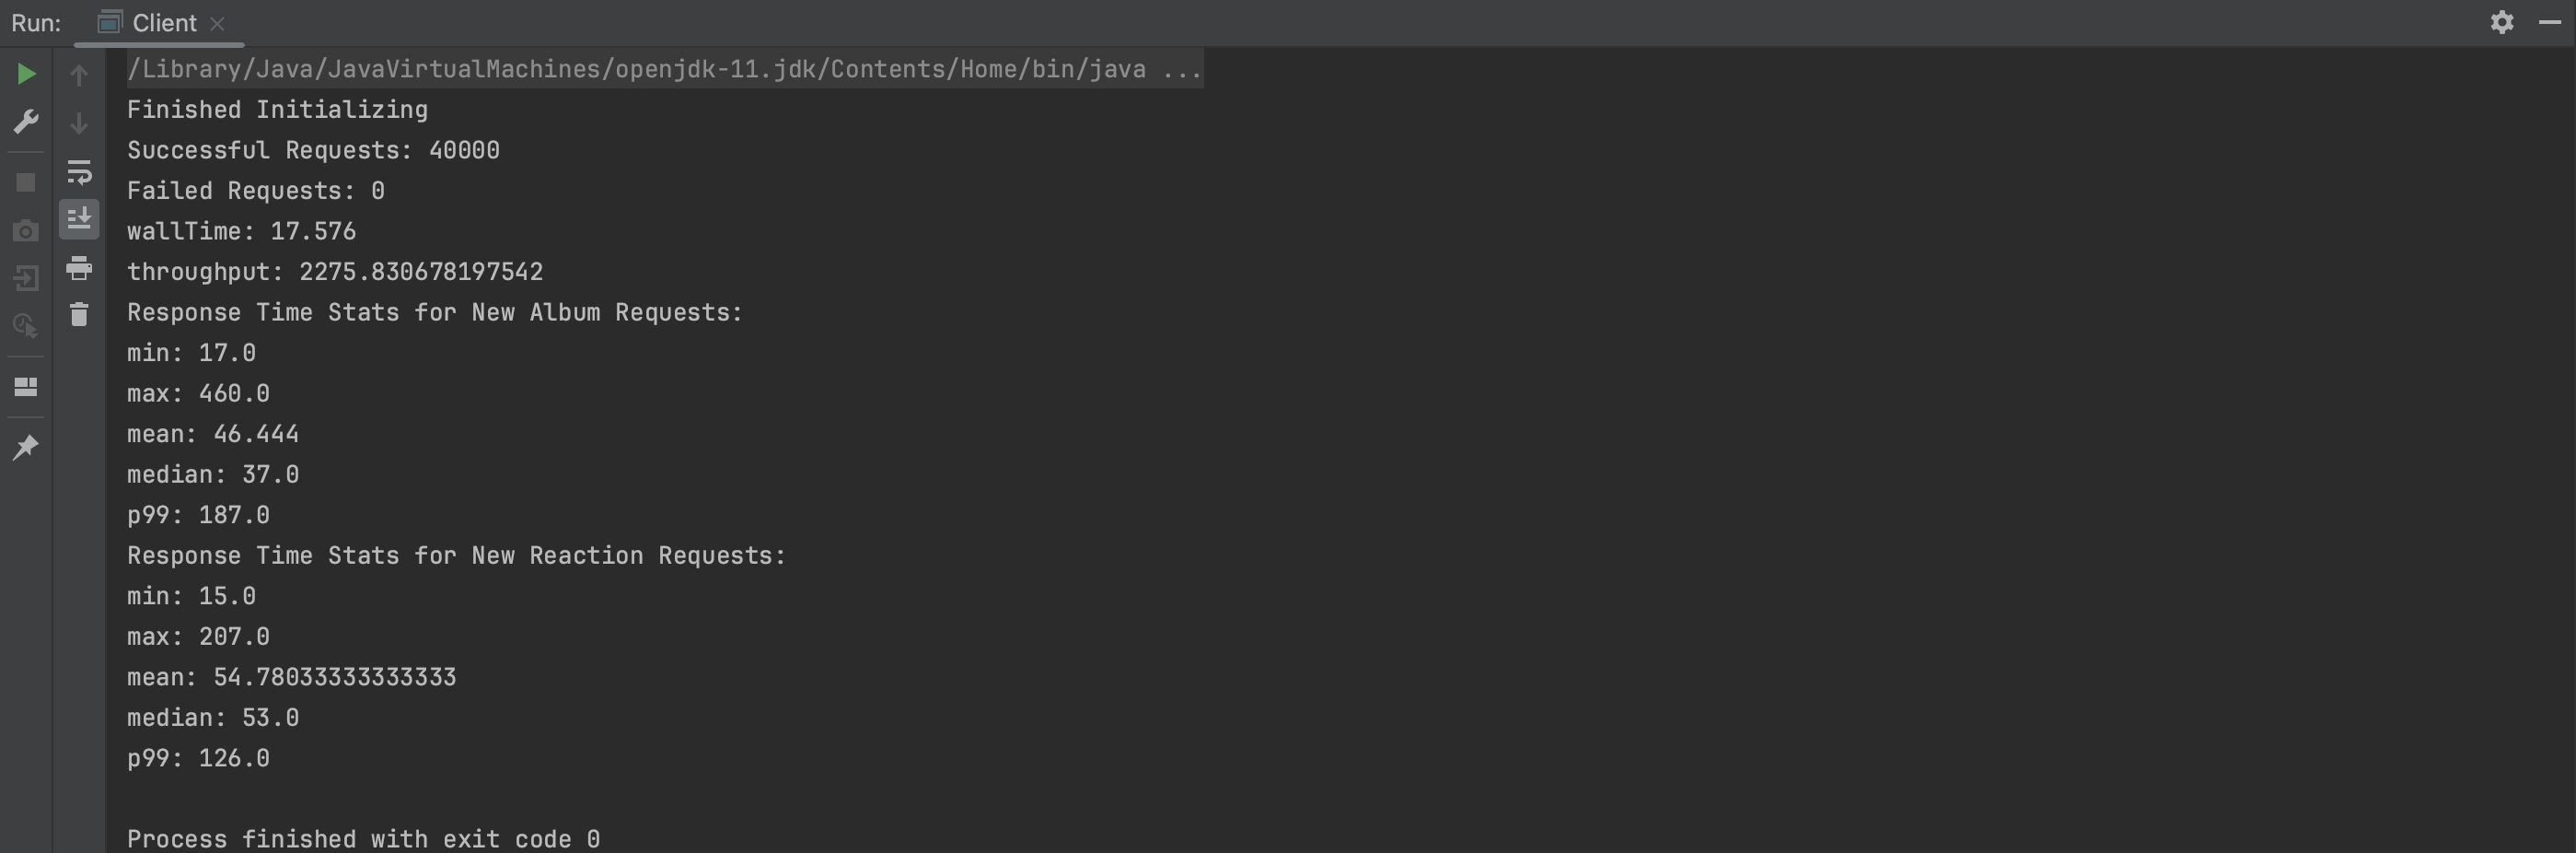
\includegraphics[width=\textwidth]{images/stats_10.png}
    \caption{Single Servlet - threadGroupSize = 10, numThreadGroups = 10, delay = 2, consumers=10}
\end{figure}
\begin{figure}[H]
    \centering
    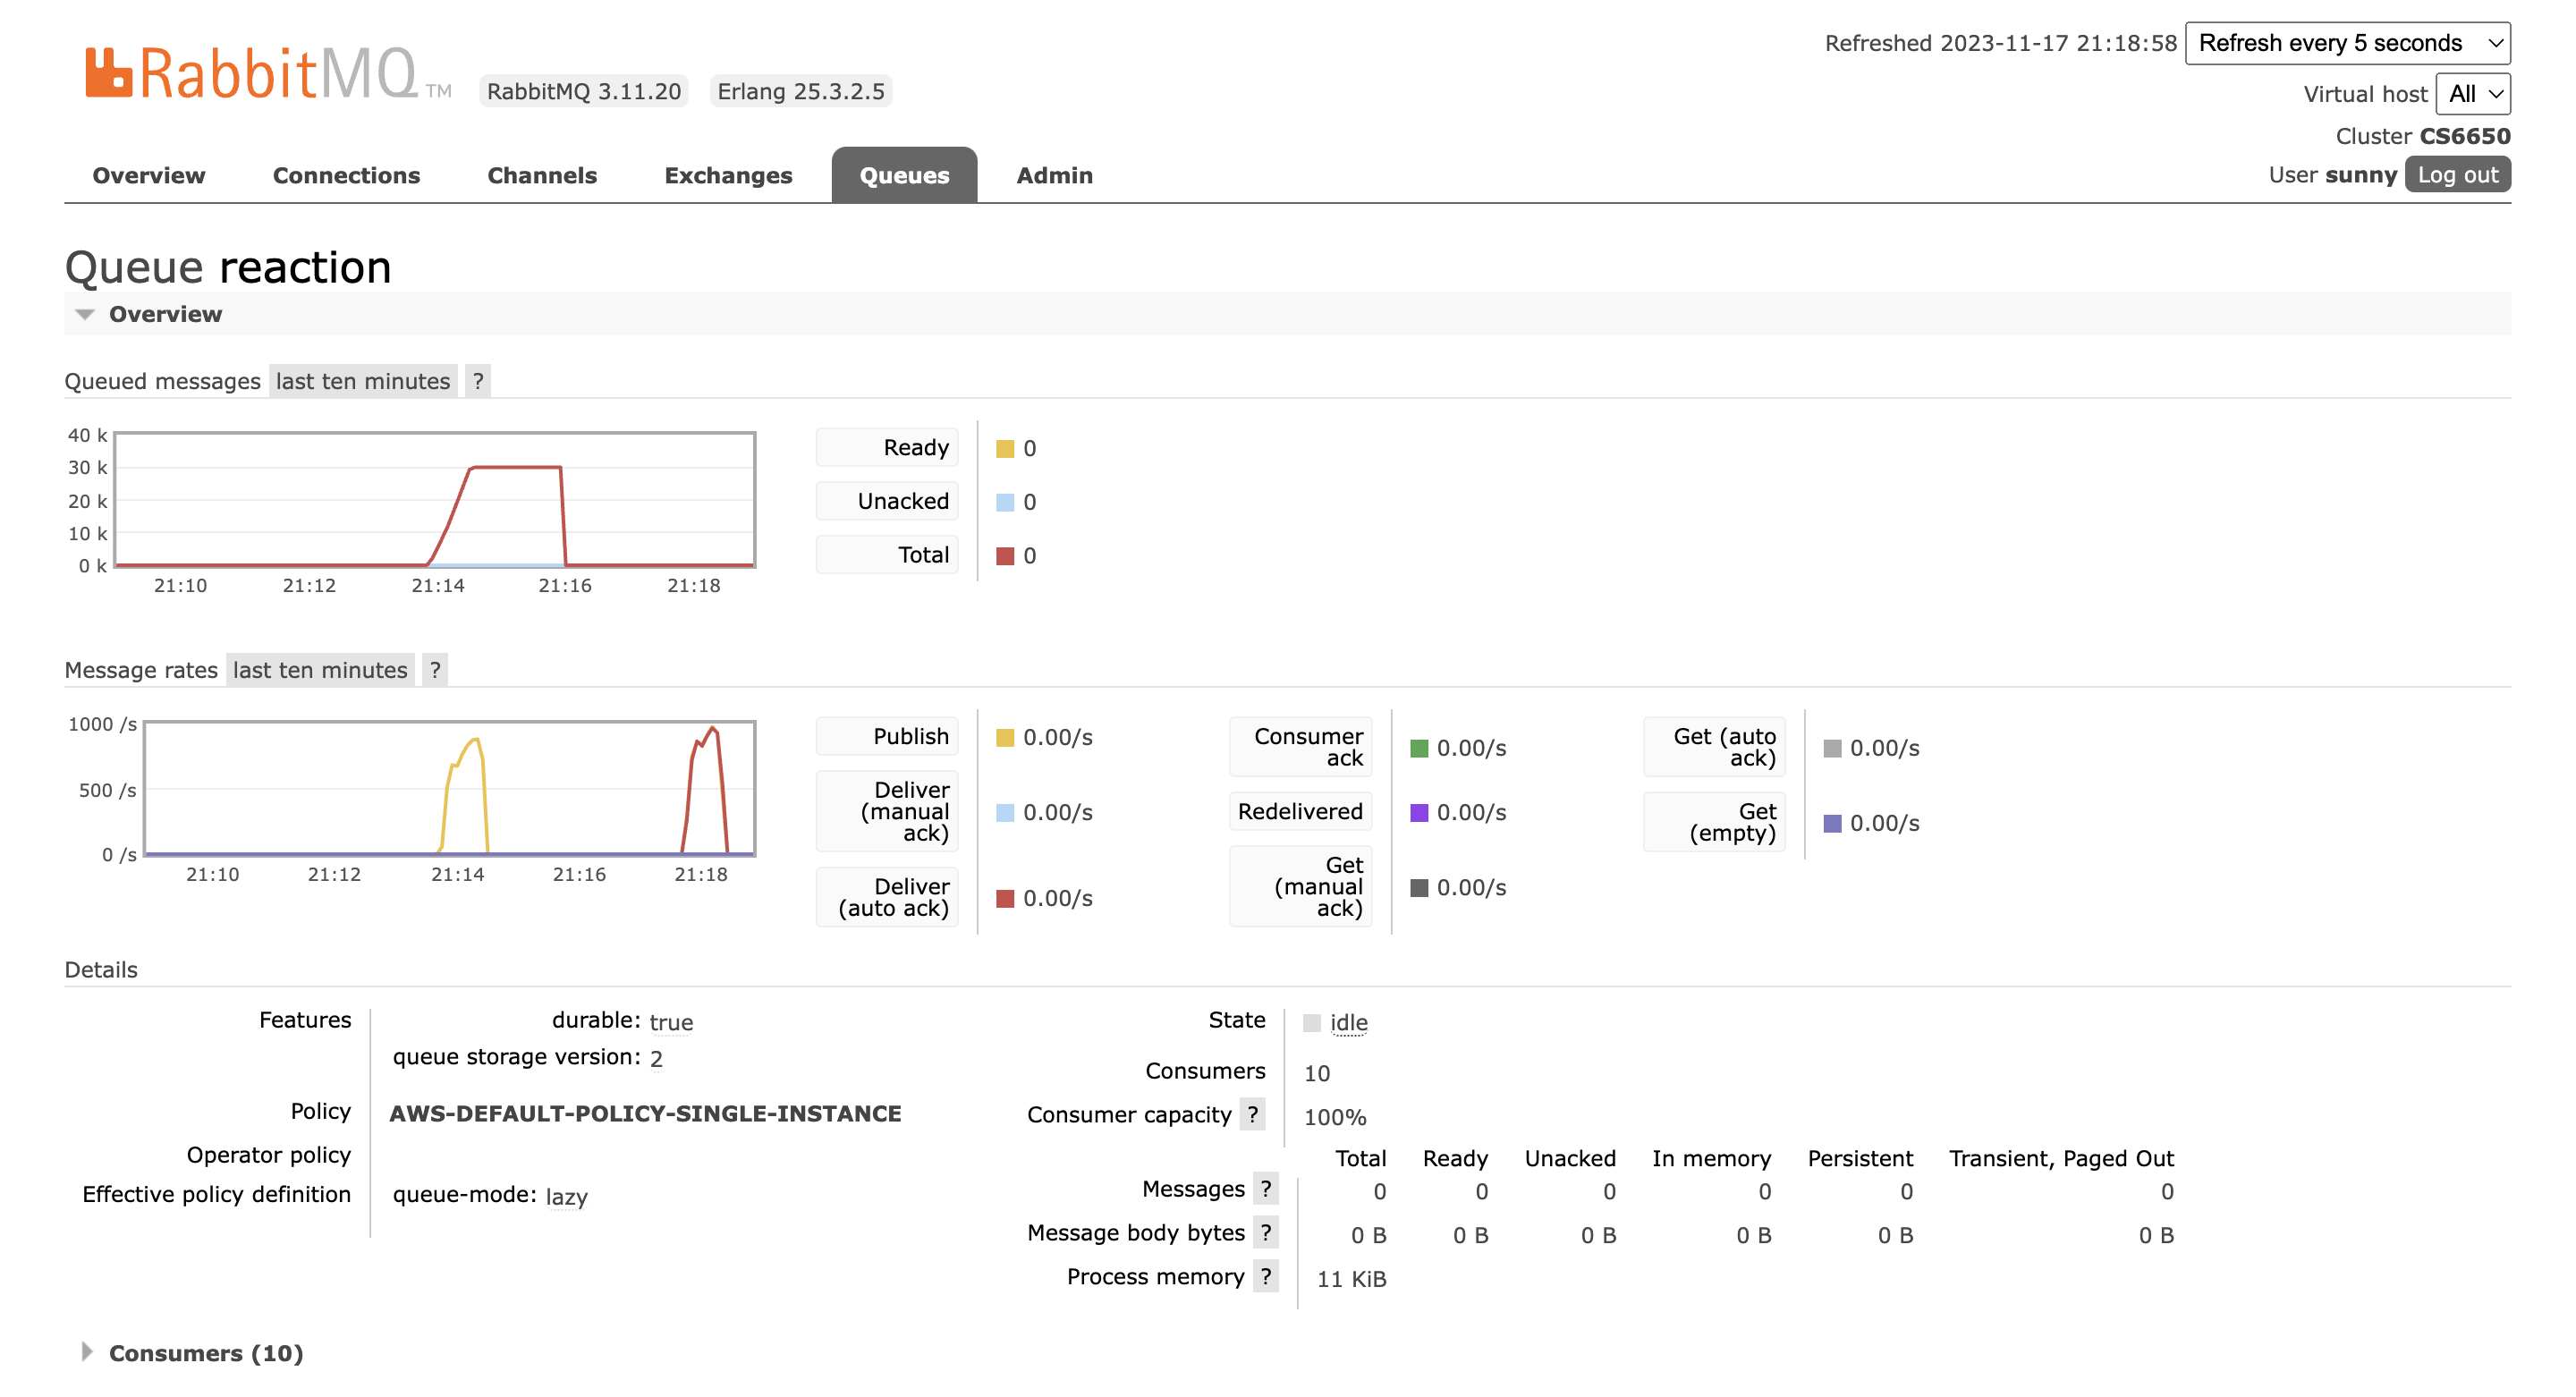
\includegraphics[width=\textwidth]{images/mq_console_10.png}
    \caption{MQ Console - threadGroupSize = 10, numThreadGroups = 10, delay = 2, consumers=10 (The run around 21:18)}
\end{figure}
\begin{figure}[H]
    \centering
    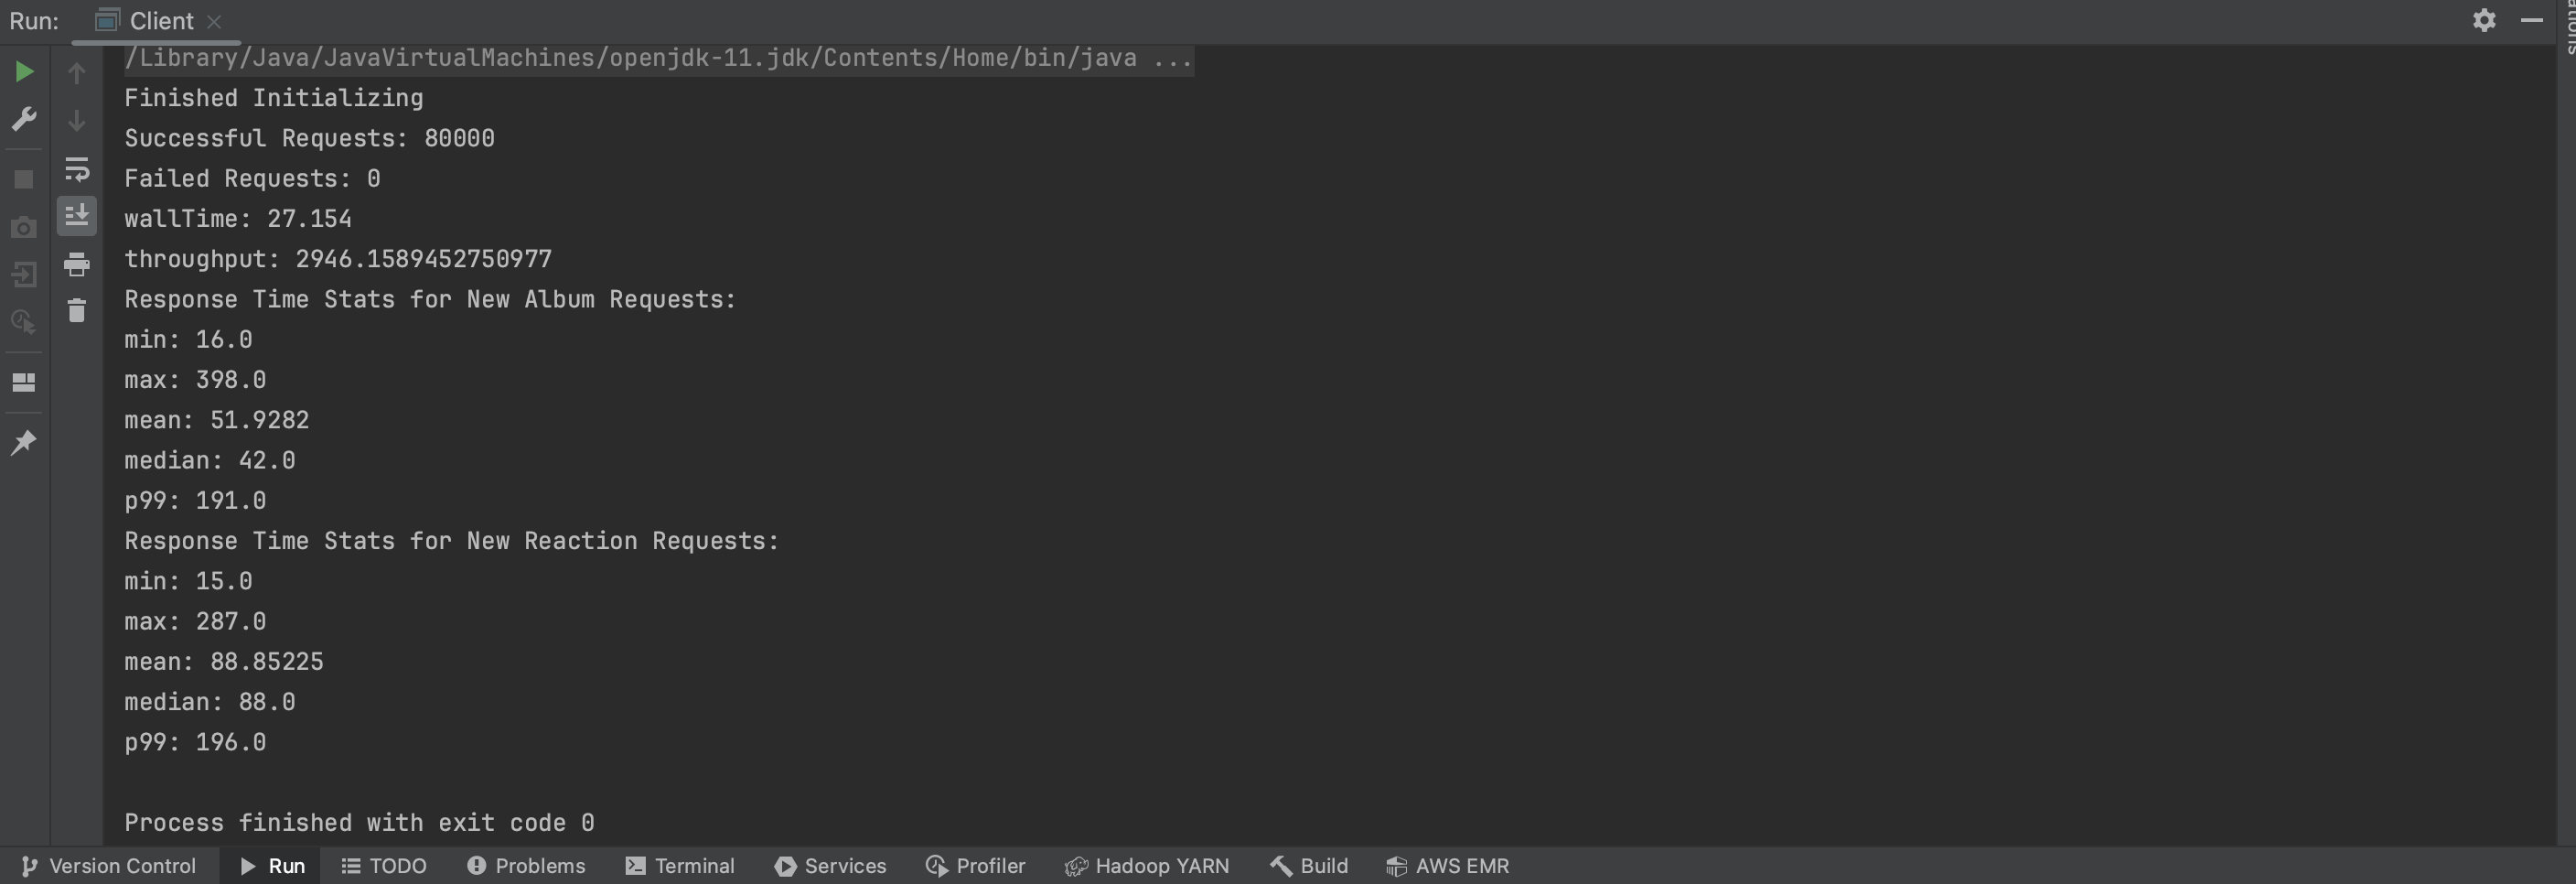
\includegraphics[width=\textwidth]{images/stats_20.png}
    \caption{Single Servlet - threadGroupSize = 10, numThreadGroups = 20, delay = 2, consumers=10}
\end{figure}
\begin{figure}[H]
    \centering
    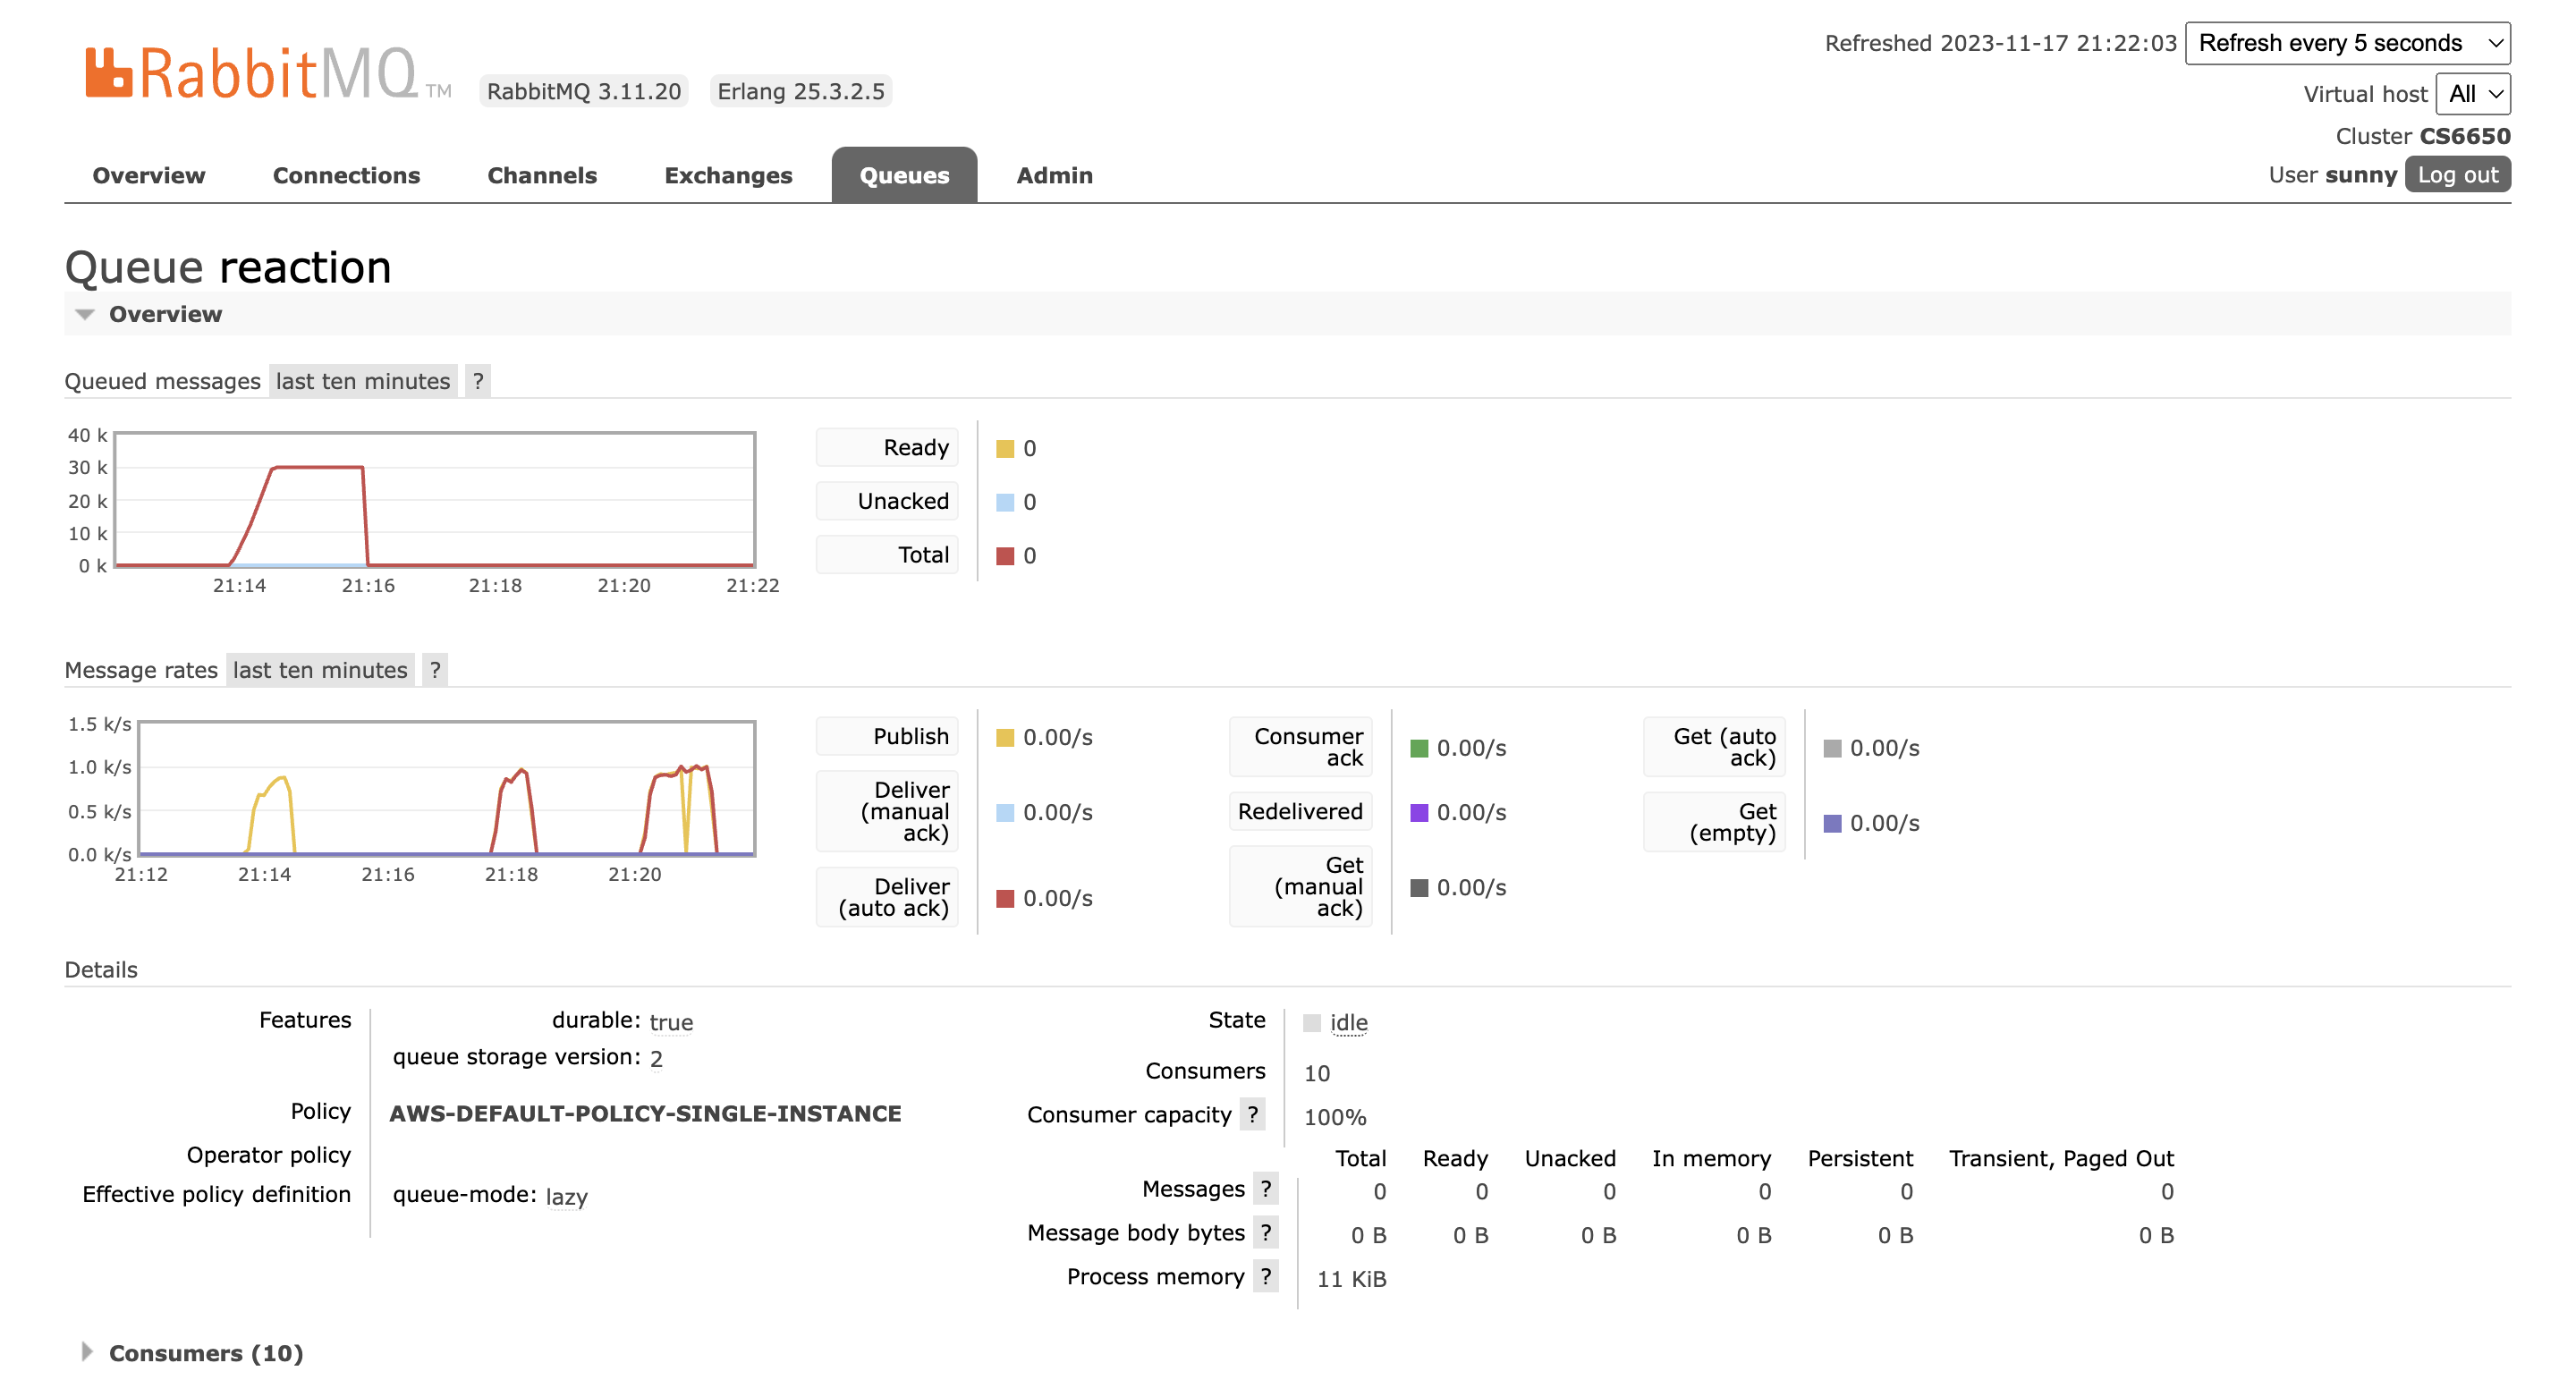
\includegraphics[width=\textwidth]{images/mq_console_20.png}
    \caption{MQ Console - threadGroupSize = 10, numThreadGroups = 20, delay = 2, consumers=10}
\end{figure}
\begin{figure}[H]
    \centering
    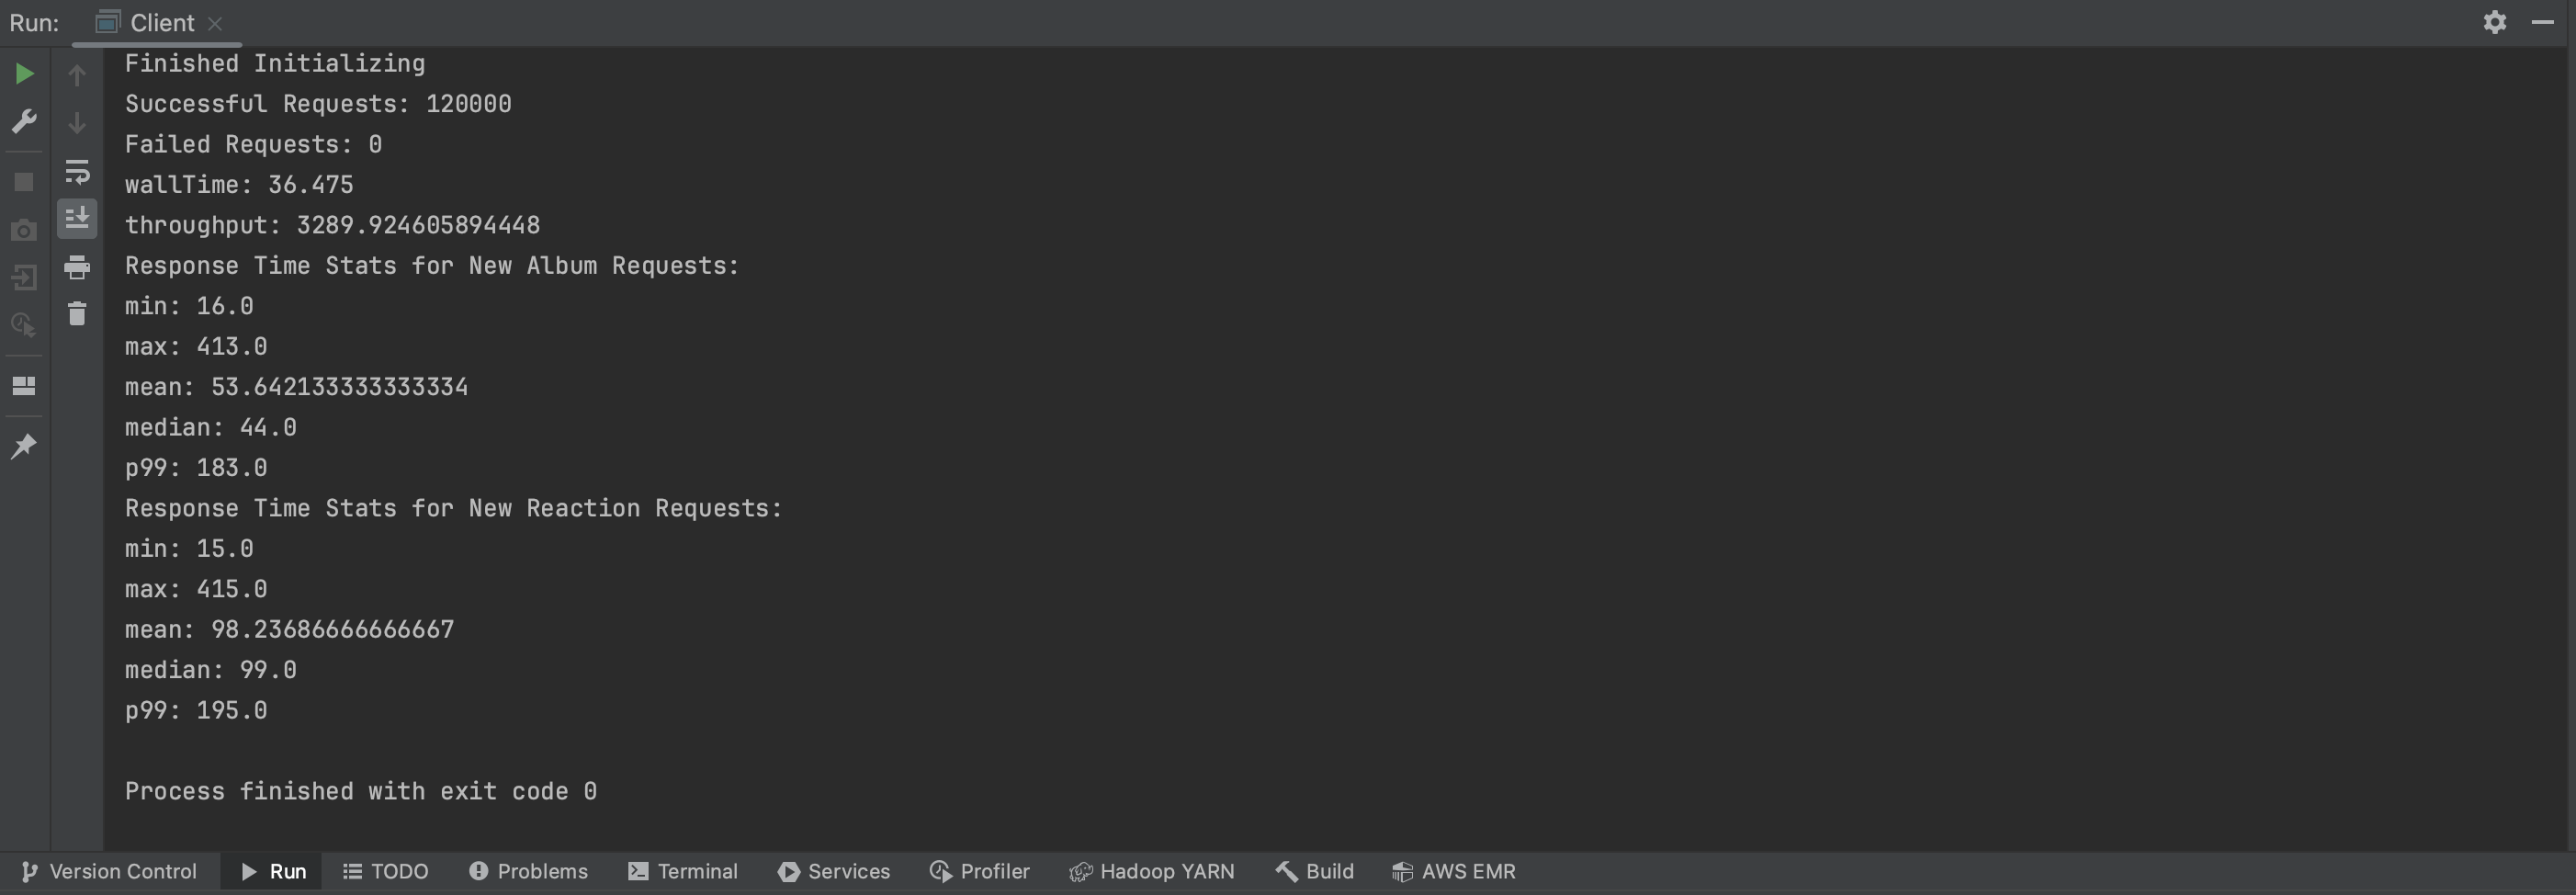
\includegraphics[width=\textwidth]{images/stats_30.png}
    \caption{Single Servlet - threadGroupSize = 10, numThreadGroups = 30, delay = 2, consumers=10}
\end{figure}
\begin{figure}[H]
    \centering
    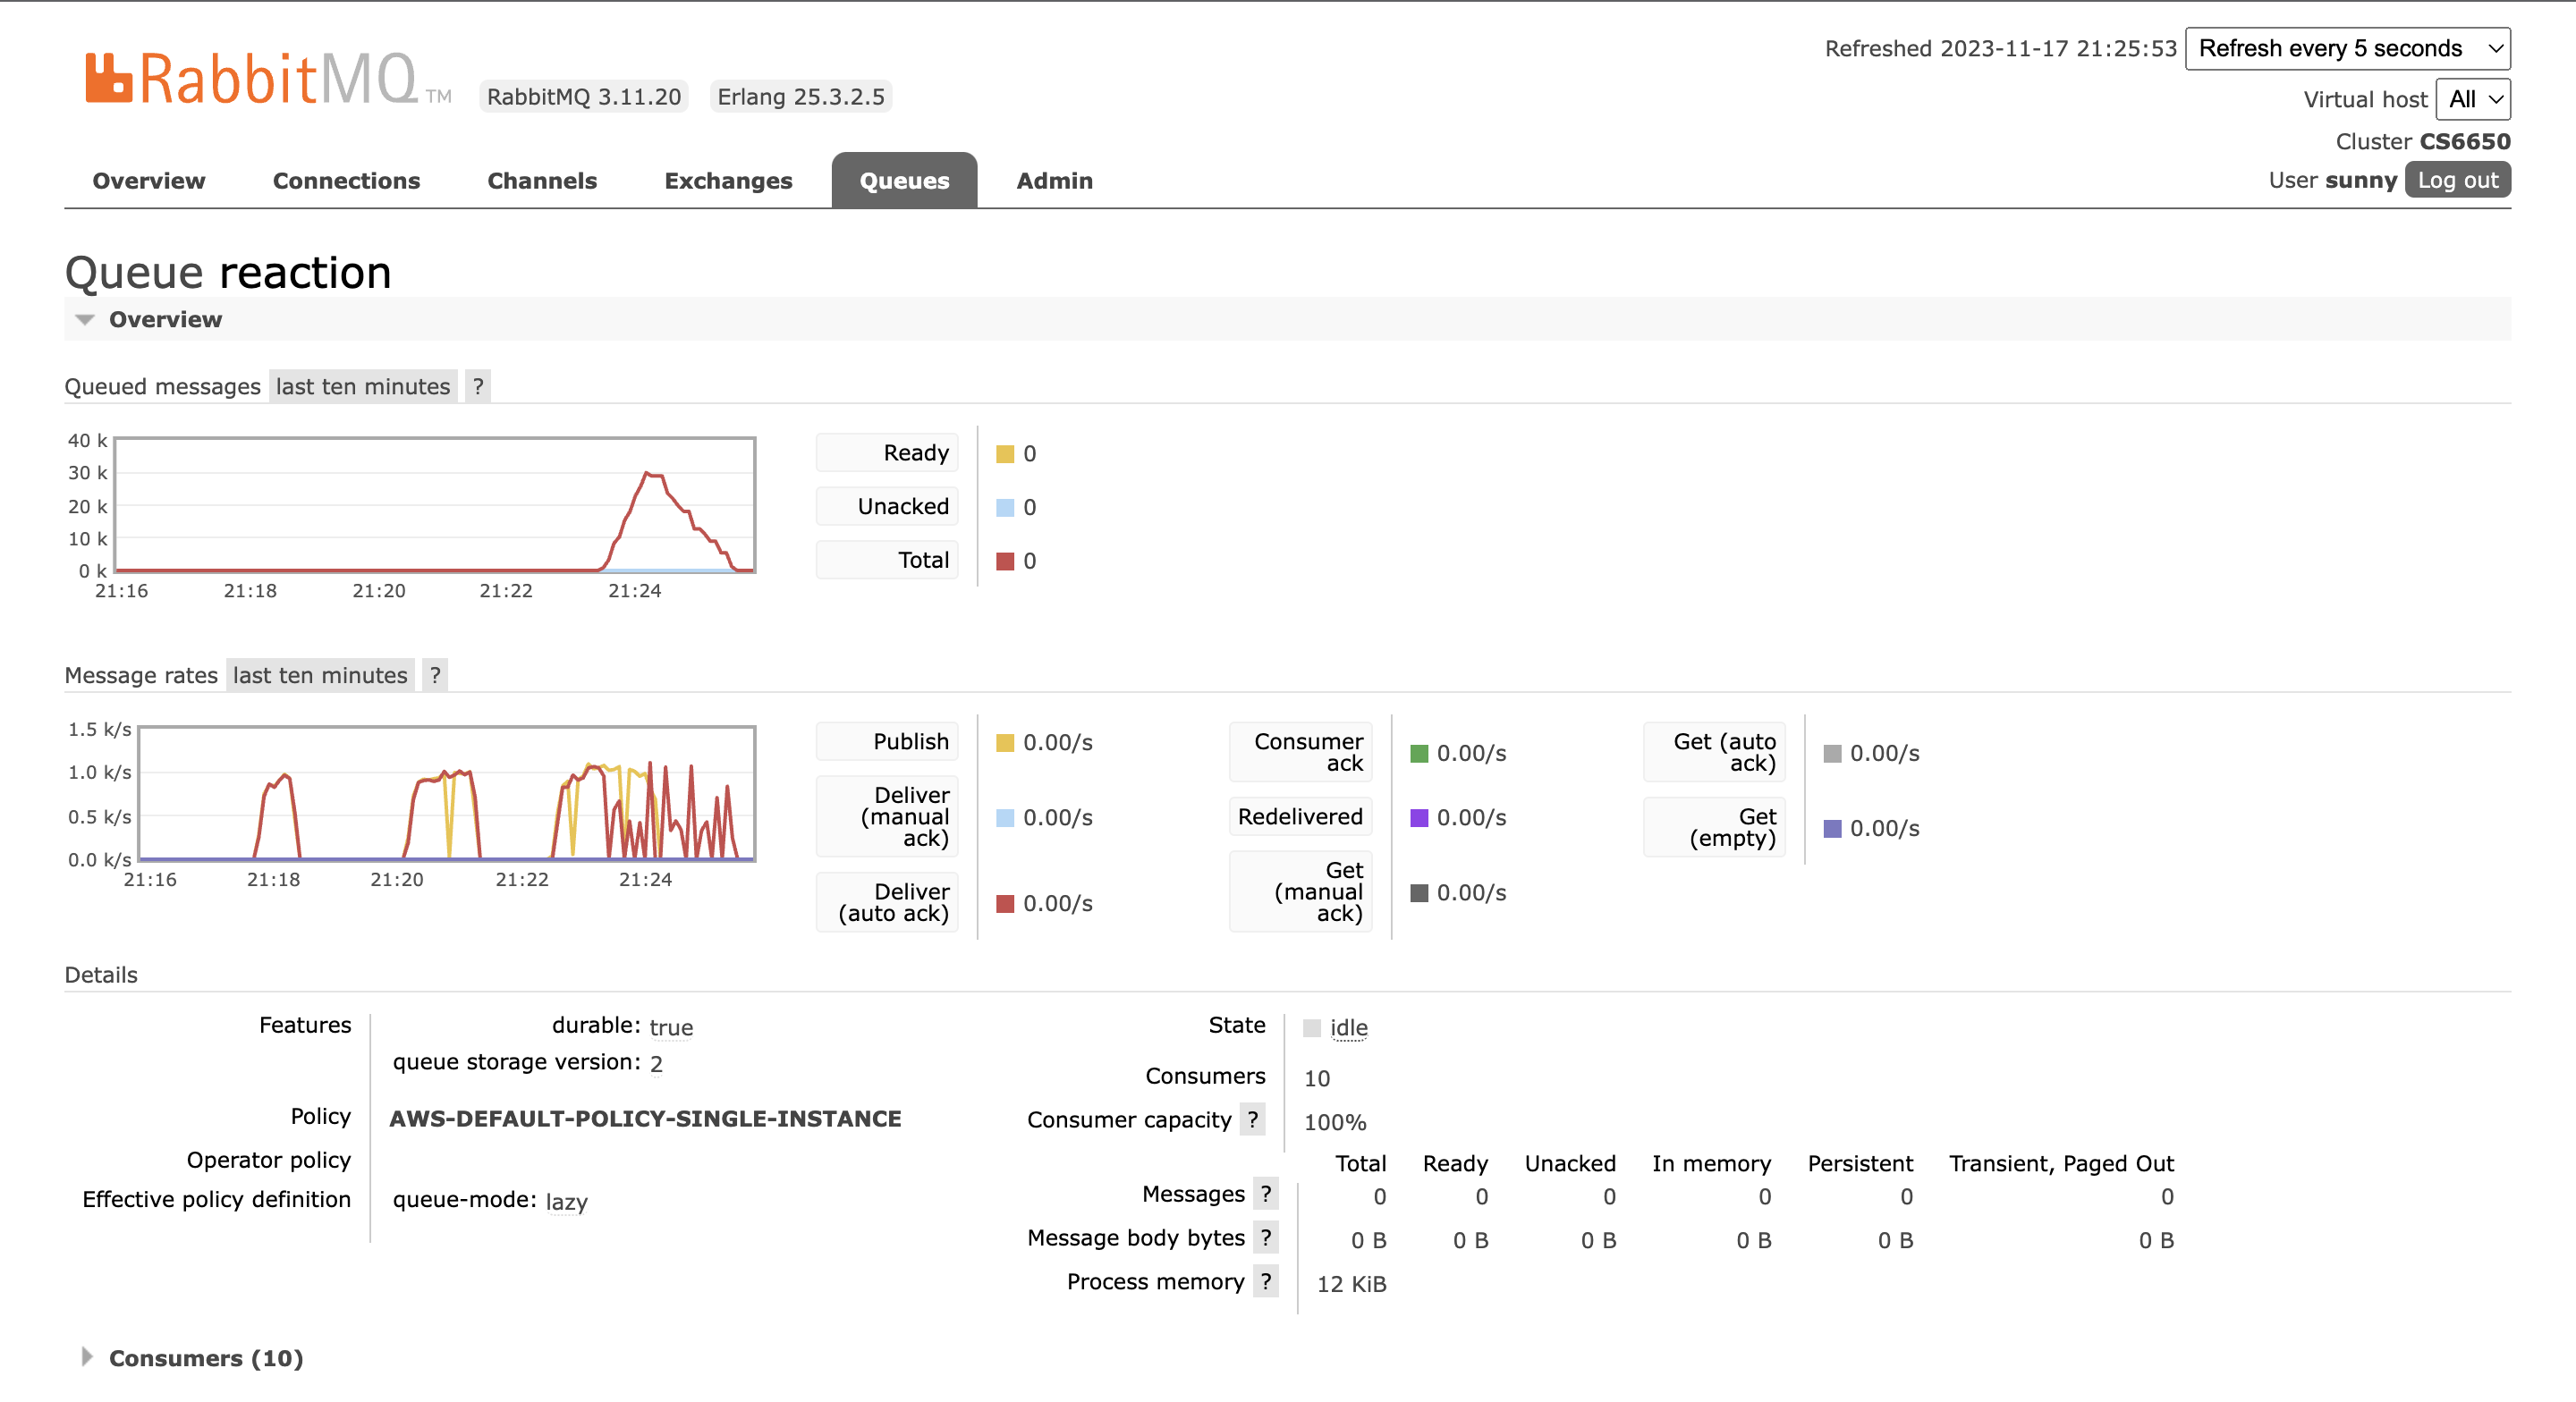
\includegraphics[width=\textwidth]{images/mq_console_30.png}
    \caption{MQ Console - threadGroupSize = 10, numThreadGroups = 30, delay = 2, consumers=10}
\end{figure}


\begin{table}[H]
    \begin{tabular}{|cc|ccc|}
    \hline
    \multicolumn{2}{|c|}{}                                              & \multicolumn{3}{c|}{Single Servlet}                                   \\ \hline
    \multicolumn{2}{|c|}{Configuration}                                 & \multicolumn{1}{c|}{10/10/2} & \multicolumn{1}{c|}{10/20/2} & 10/30/2 \\ \hline
    \multicolumn{2}{|c|}{Wall Time}                                     & \multicolumn{1}{c|}{18}      & \multicolumn{1}{c|}{27}      & 36      \\ \hline
    \multicolumn{2}{|c|}{Throughput}                                    & \multicolumn{1}{c|}{2276}    & \multicolumn{1}{c|}{2946}    & 3290    \\ \hline
    \multicolumn{1}{|c|}{\multirow{5}{*}{Post Album}}          & Min    & \multicolumn{1}{c|}{17}      & \multicolumn{1}{c|}{16}      & 16      \\ \cline{2-5} 
    \multicolumn{1}{|c|}{}                                     & Max    & \multicolumn{1}{c|}{460}     & \multicolumn{1}{c|}{398}     & 413     \\ \cline{2-5} 
    \multicolumn{1}{|c|}{}                                     & Mean   & \multicolumn{1}{c|}{46}      & \multicolumn{1}{c|}{52}      & 54      \\ \cline{2-5} 
    \multicolumn{1}{|c|}{}                                     & Median & \multicolumn{1}{c|}{37}      & \multicolumn{1}{c|}{42}      & 44      \\ \cline{2-5} 
    \multicolumn{1}{|c|}{}                                     & P99    & \multicolumn{1}{c|}{187}     & \multicolumn{1}{c|}{191}     & 183     \\ \hline
    \multicolumn{1}{|c|}{\multirow{5}{*}{Post Album Reaction}} & Min    & \multicolumn{1}{c|}{15}      & \multicolumn{1}{c|}{15}      & 15      \\ \cline{2-5} 
    \multicolumn{1}{|c|}{}                                     & Max    & \multicolumn{1}{c|}{207}     & \multicolumn{1}{c|}{287}     & 415     \\ \cline{2-5} 
    \multicolumn{1}{|c|}{}                                     & Mean   & \multicolumn{1}{c|}{55}      & \multicolumn{1}{c|}{89}      & 98      \\ \cline{2-5} 
    \multicolumn{1}{|c|}{}                                     & Median & \multicolumn{1}{c|}{53}      & \multicolumn{1}{c|}{88}      & 99      \\ \cline{2-5} 
    \multicolumn{1}{|c|}{}                                     & P99    & \multicolumn{1}{c|}{126}     & \multicolumn{1}{c|}{196}     & 195     \\ \hline
    \end{tabular}
\end{table}

\newpage
In order to maximize the system throughput, I monitored the servlet's cpu utilization. In the runs above, I initialized the Executor Service to have a fixed pool of 150 threads. 
\begin{figure}[H]
    \centering
    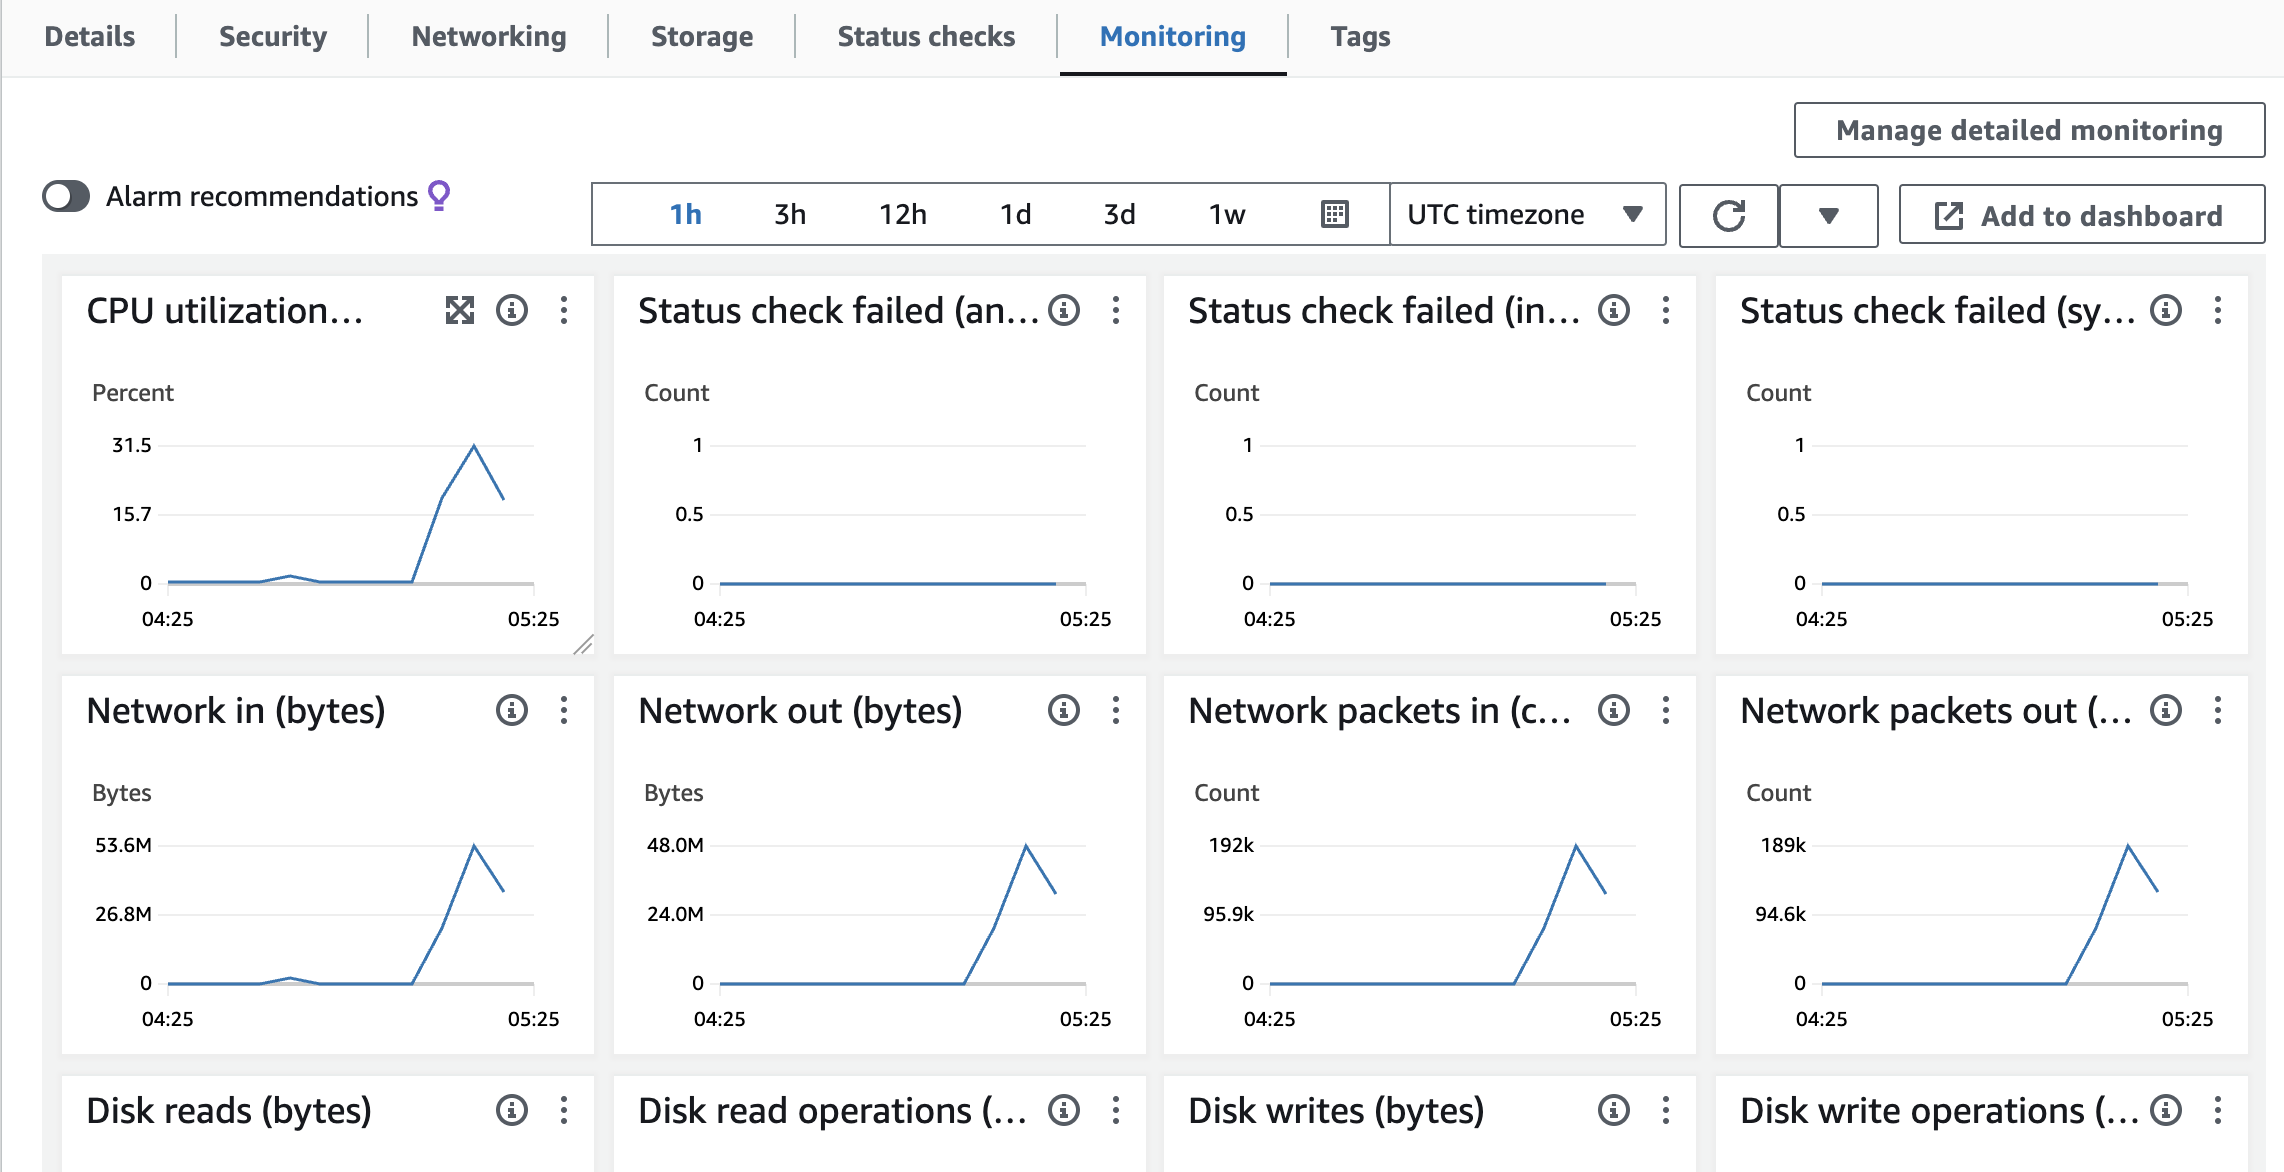
\includegraphics[width=\textwidth]{images/cpu_util.png}
    \caption{CPU Utilization when at most 150 threads firing post requests}
\end{figure}
As we can see, the cpu utilization was about 31.5\%. The server was not under heavy load, so we should be able to load the server more. I then increased the number to 200.
\begin{figure}[H]
    \centering
    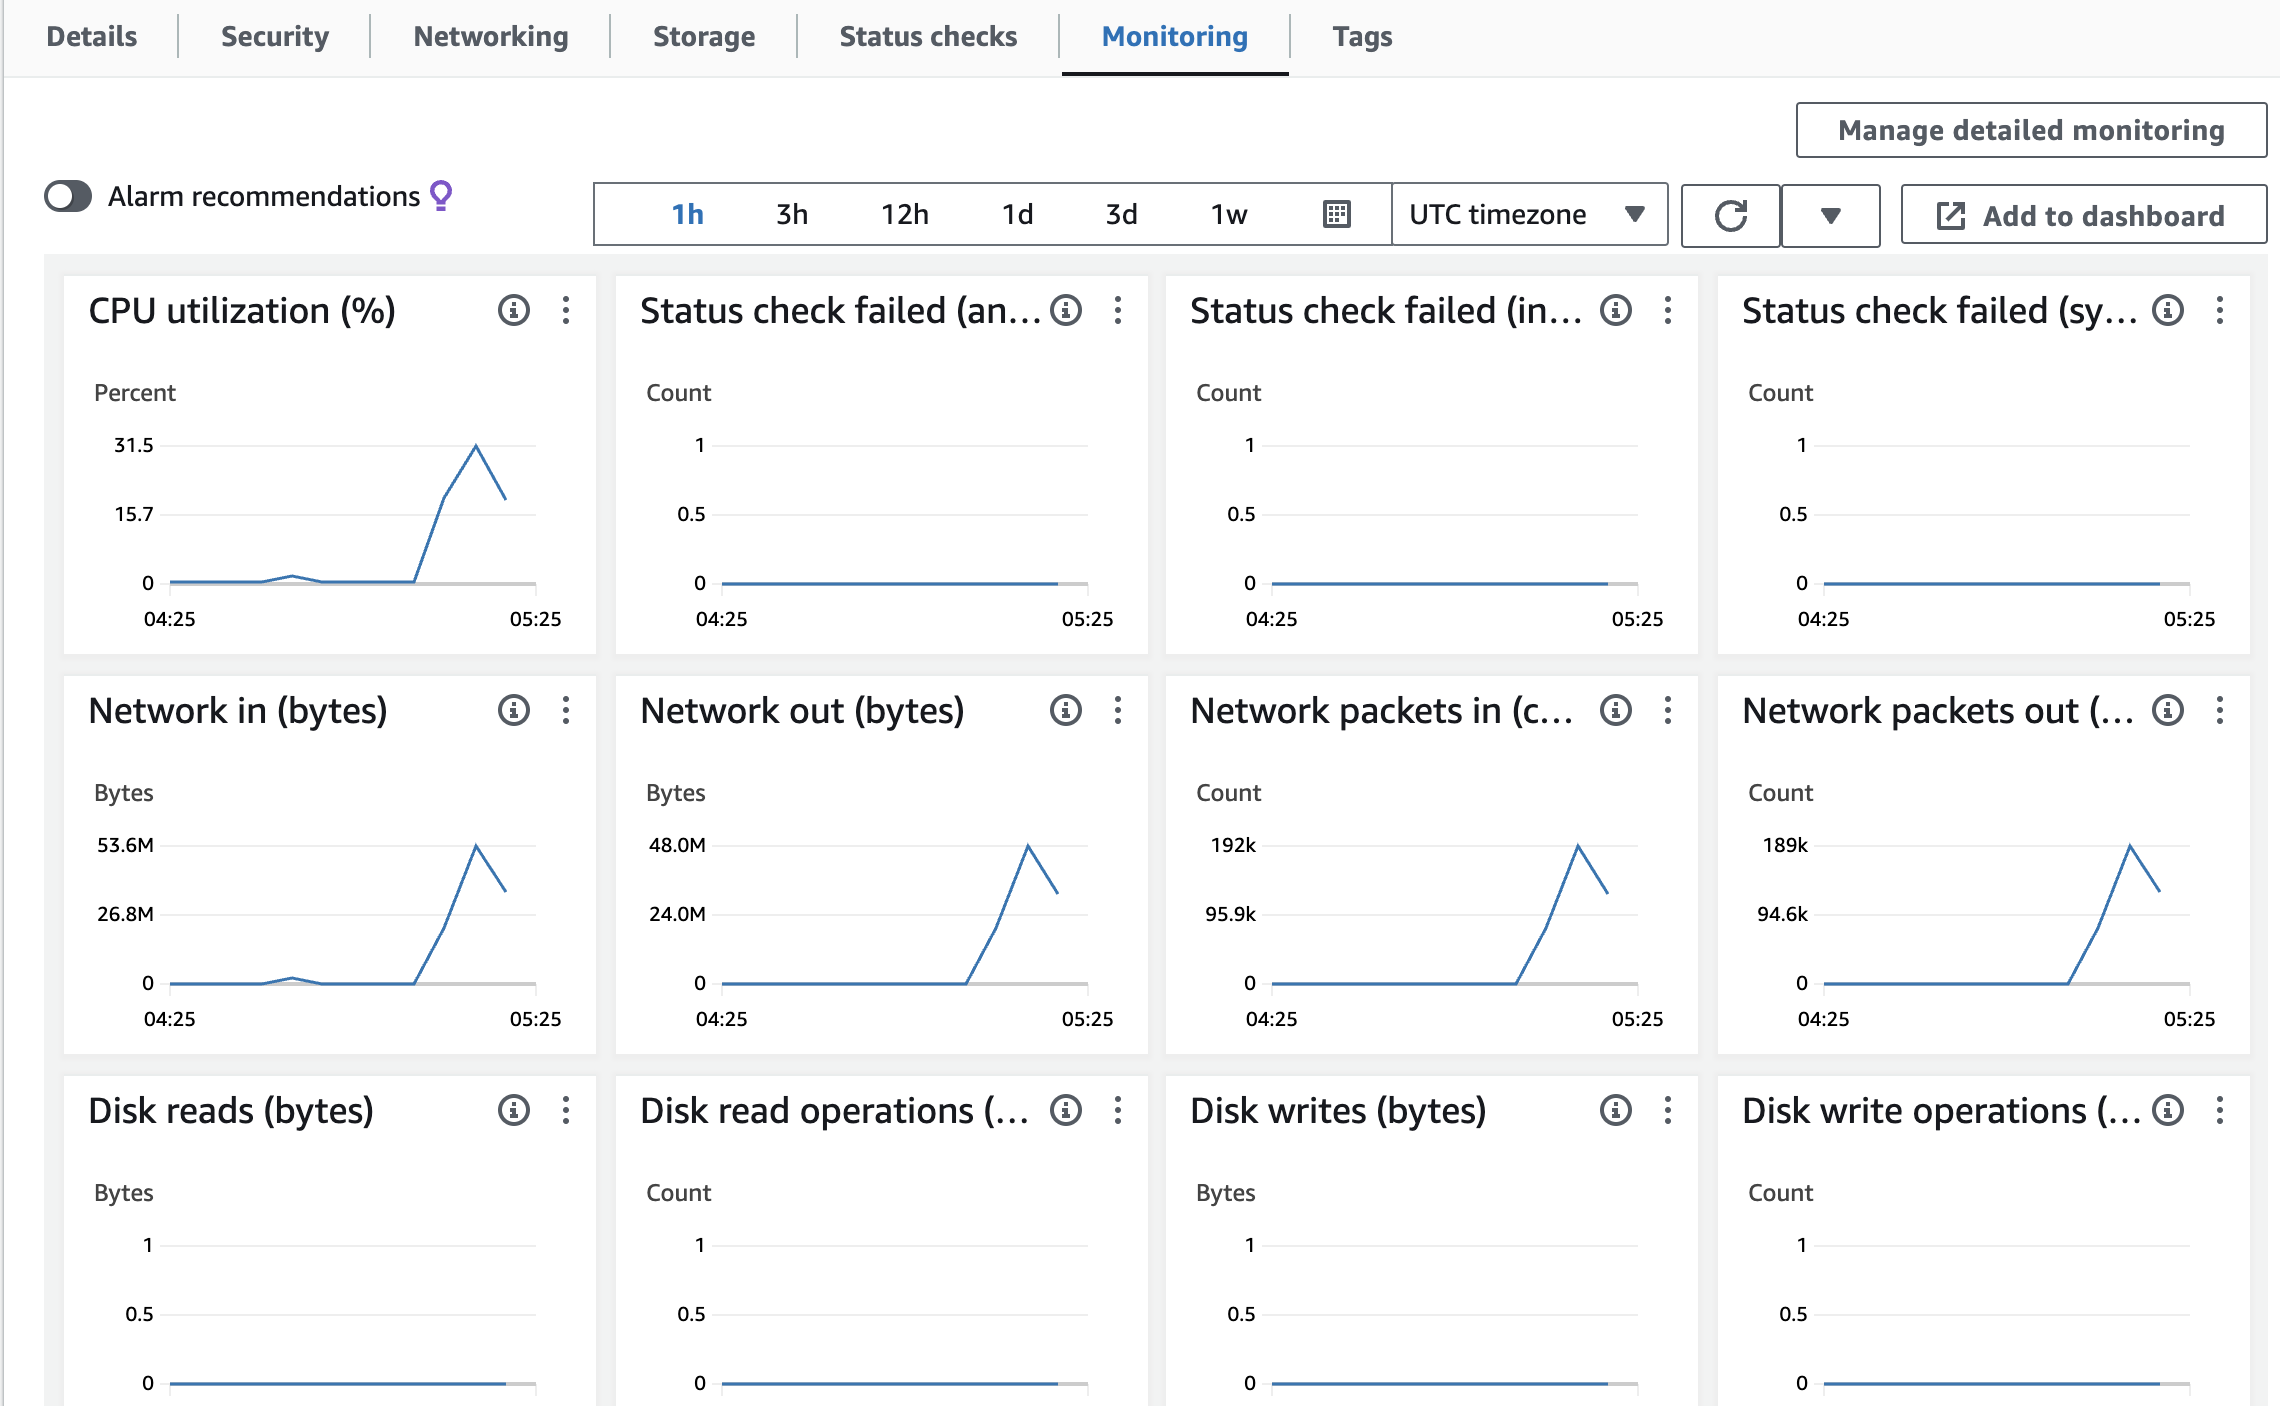
\includegraphics[width=\textwidth]{images/cpu_util_200client.png}
    \caption{CPU Utilization when at most 200 threads firing post requests}
\end{figure}
From the utilization, we see that there is no significant difference after increasing the number. This is indicating that using 150 clients already maximized the throughput. 

For the 10/30/2 configuration, we see a spike in messages queued that peaked around 30k messages. This indicates that we do not have enough consumers to process the information in time.
Therefore, I monitored the database to confirm that the database server is not overloaded.
\begin{figure}[H]
    \centering
    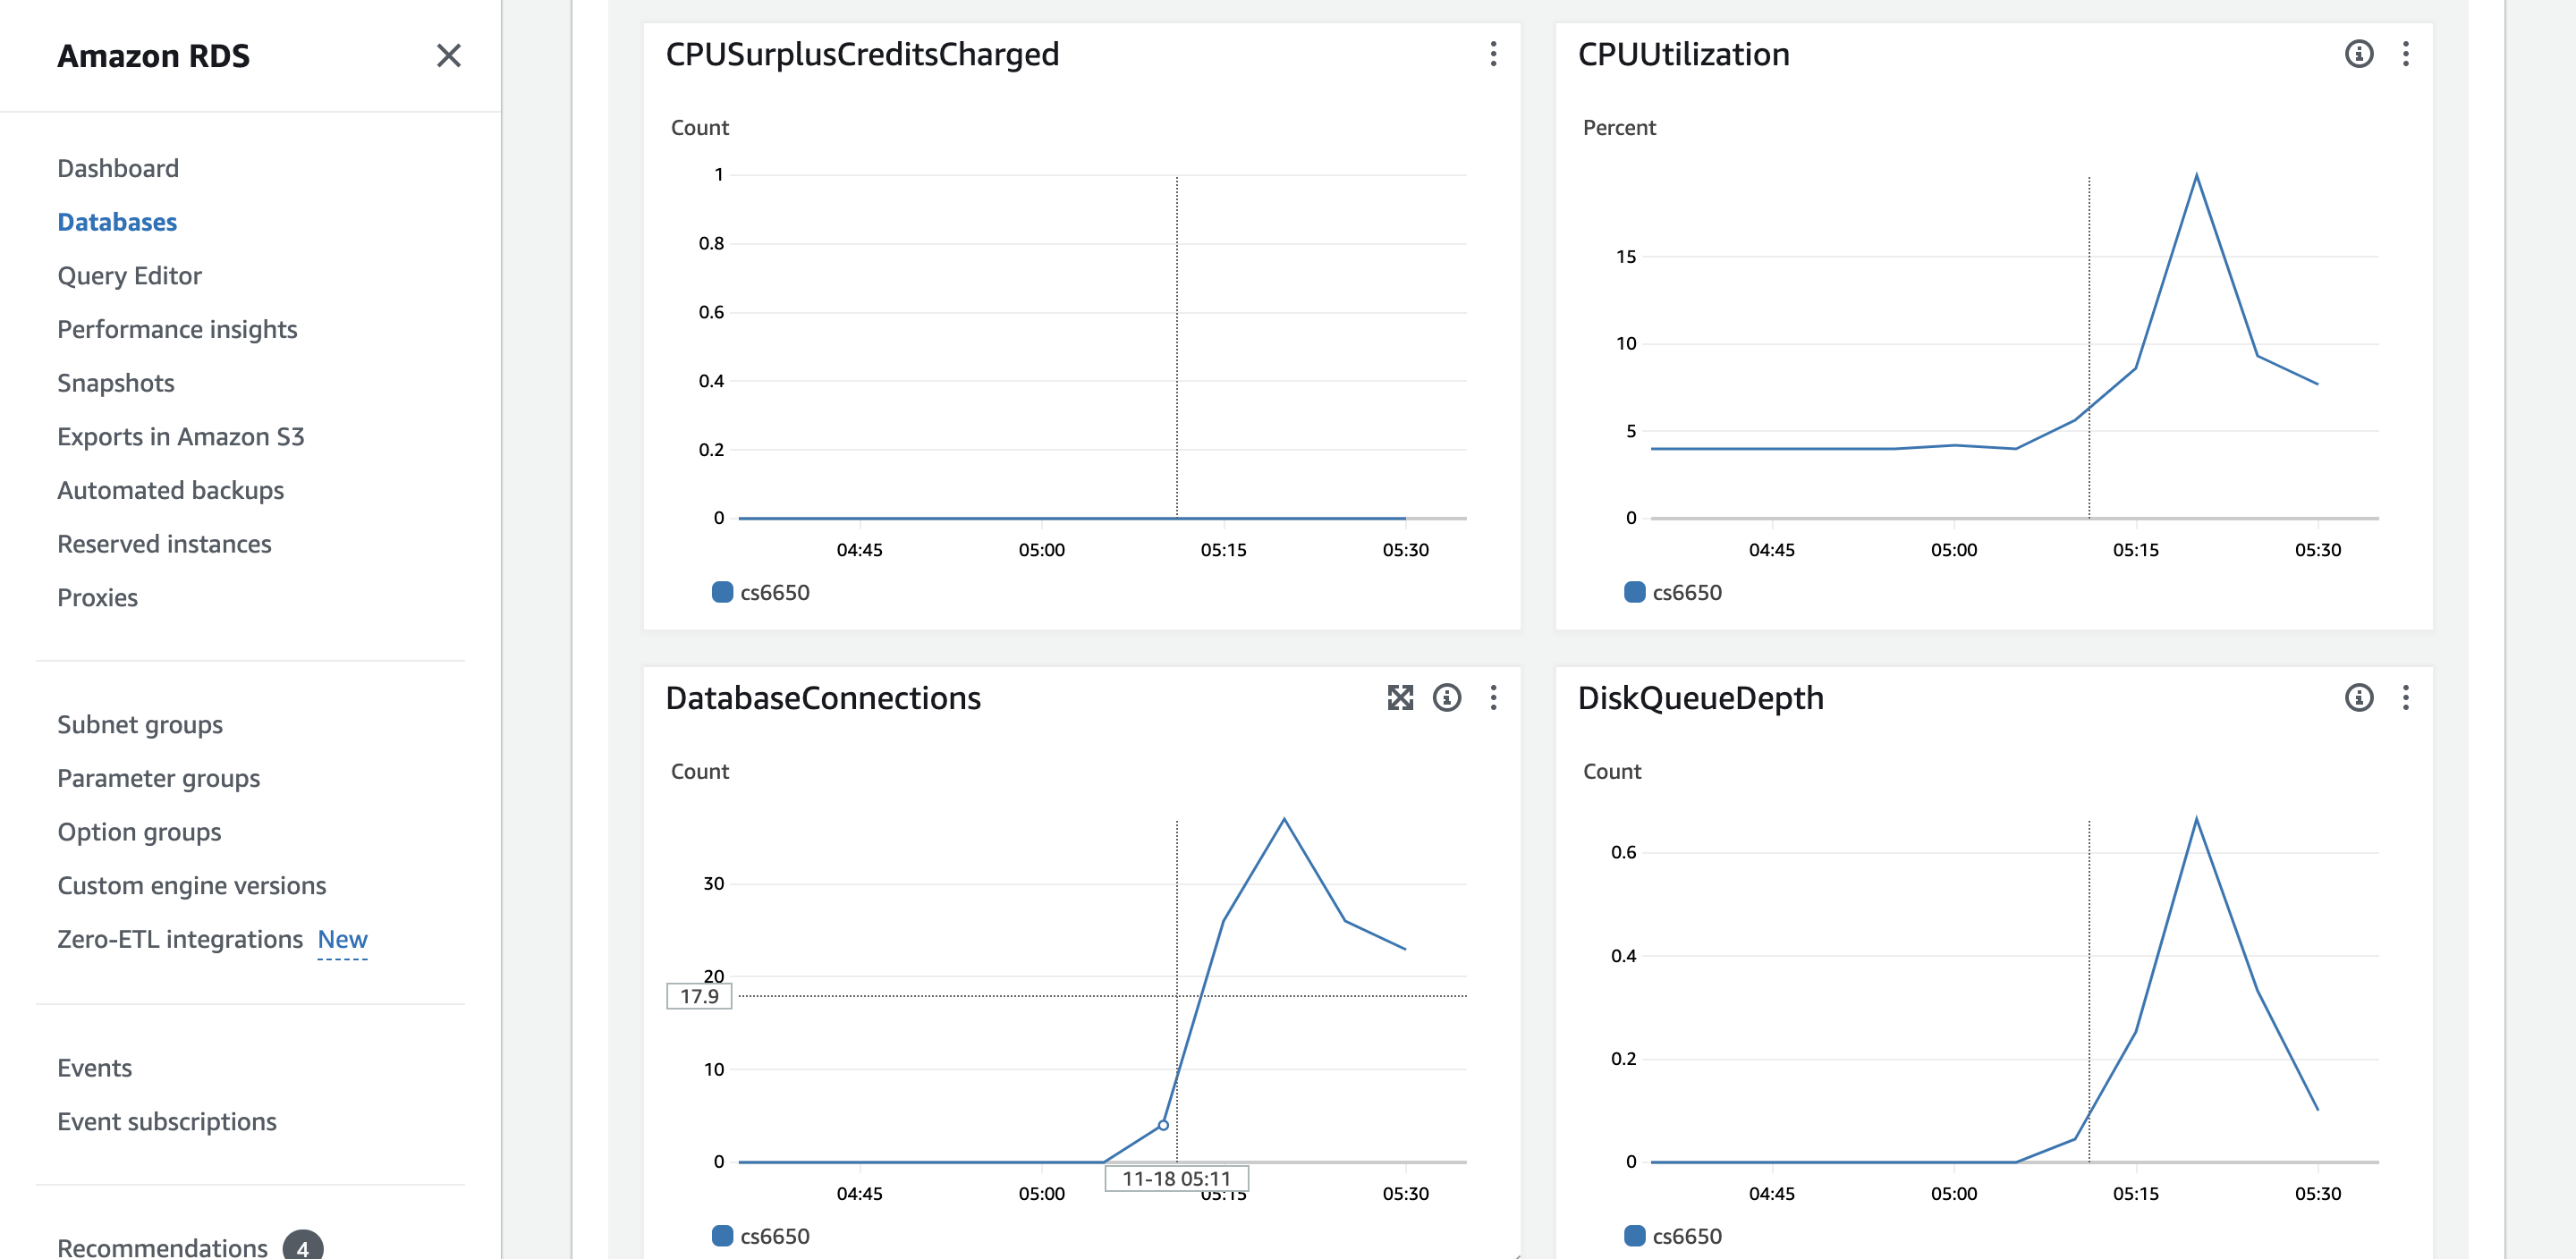
\includegraphics[width=\textwidth]{images/rds_util_connections.png}
    \caption{CPU Utilization on Database Server using 10 consumers}
\end{figure}
The cpu utilization and the number of connections are fairly low, so we can proceed to increase the number of consumers in our program.
I doubled the amount of consumers to 20.
\begin{figure}[H]
    \centering
    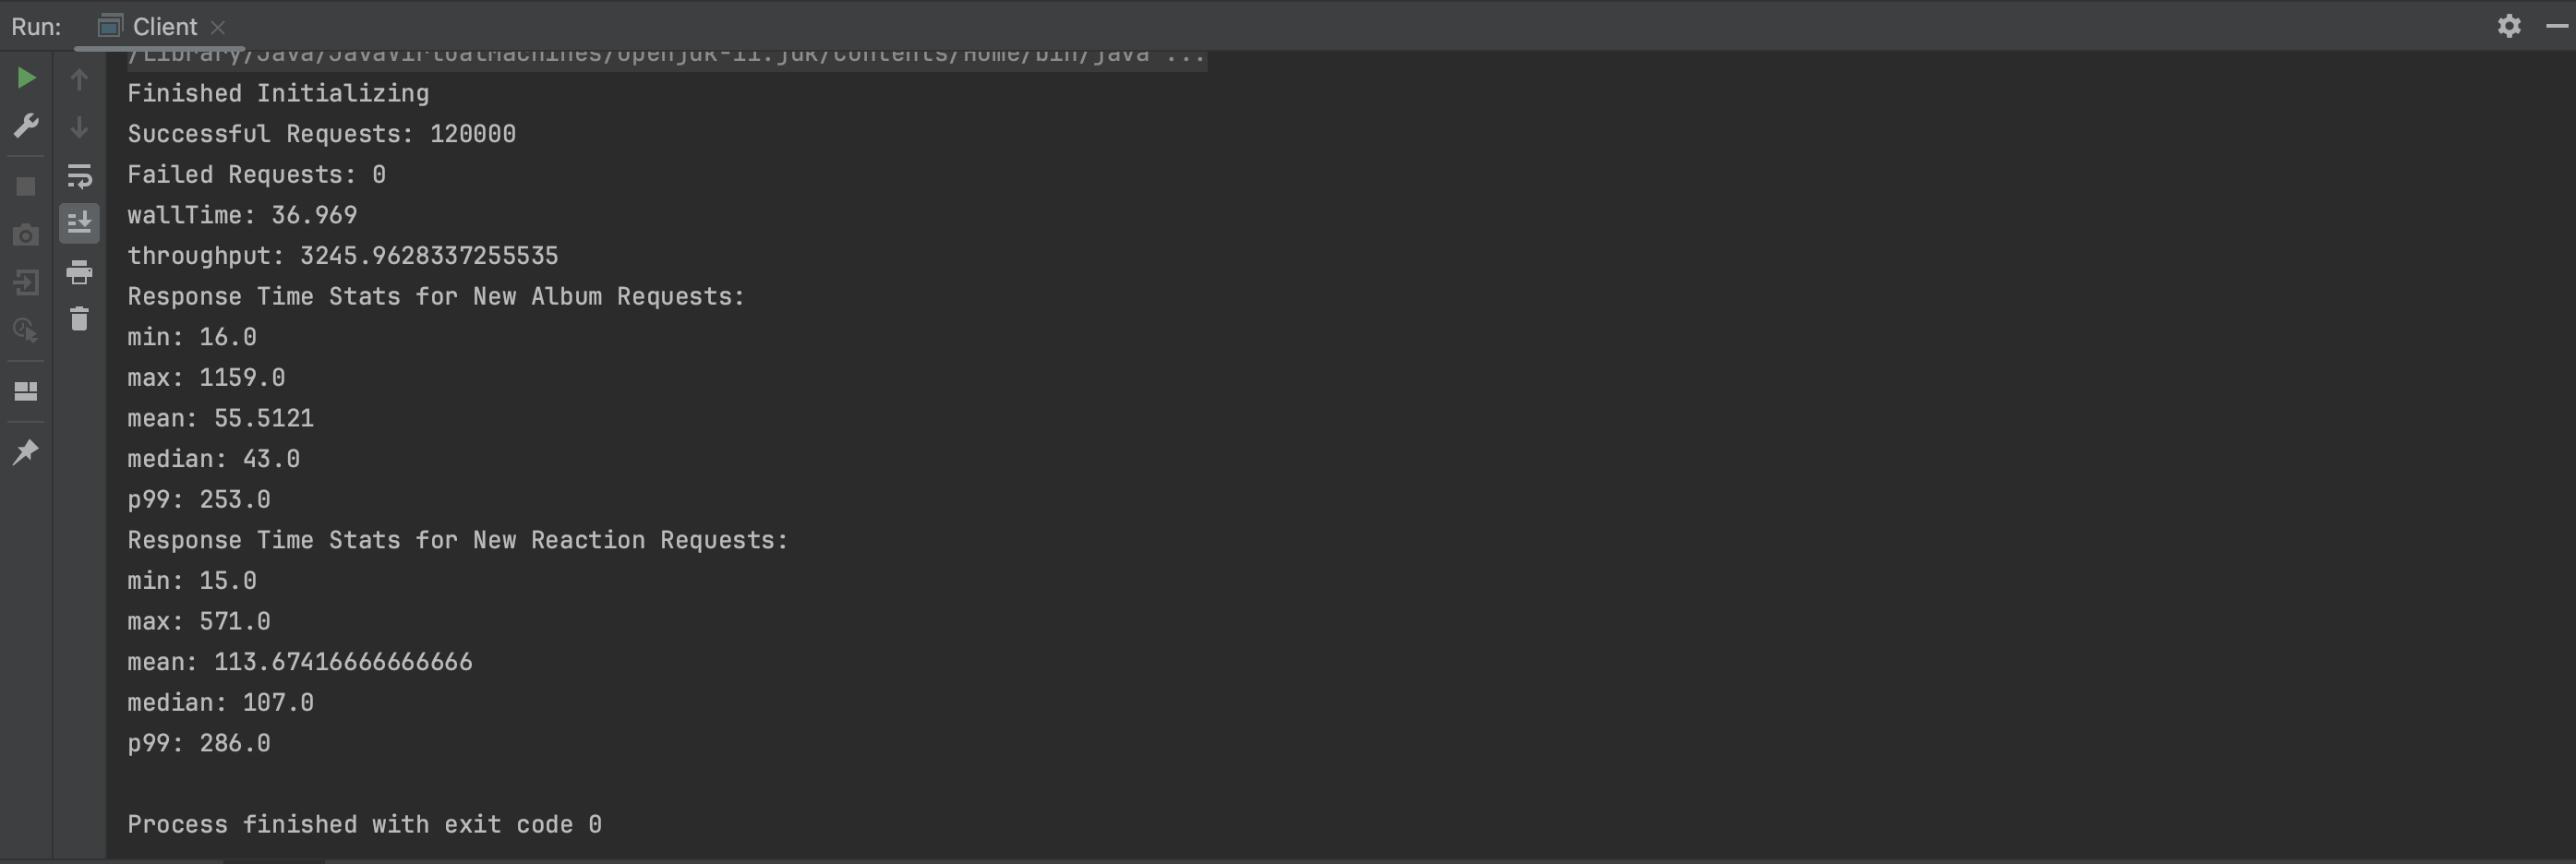
\includegraphics[width=\textwidth]{images/stats_20consumer.png}
    \caption{Single Servlet - threadGroupSize = 10, numThreadGroups = 30, delay = 2, consumers=20}
\end{figure}
\begin{figure}[H]
    \centering
    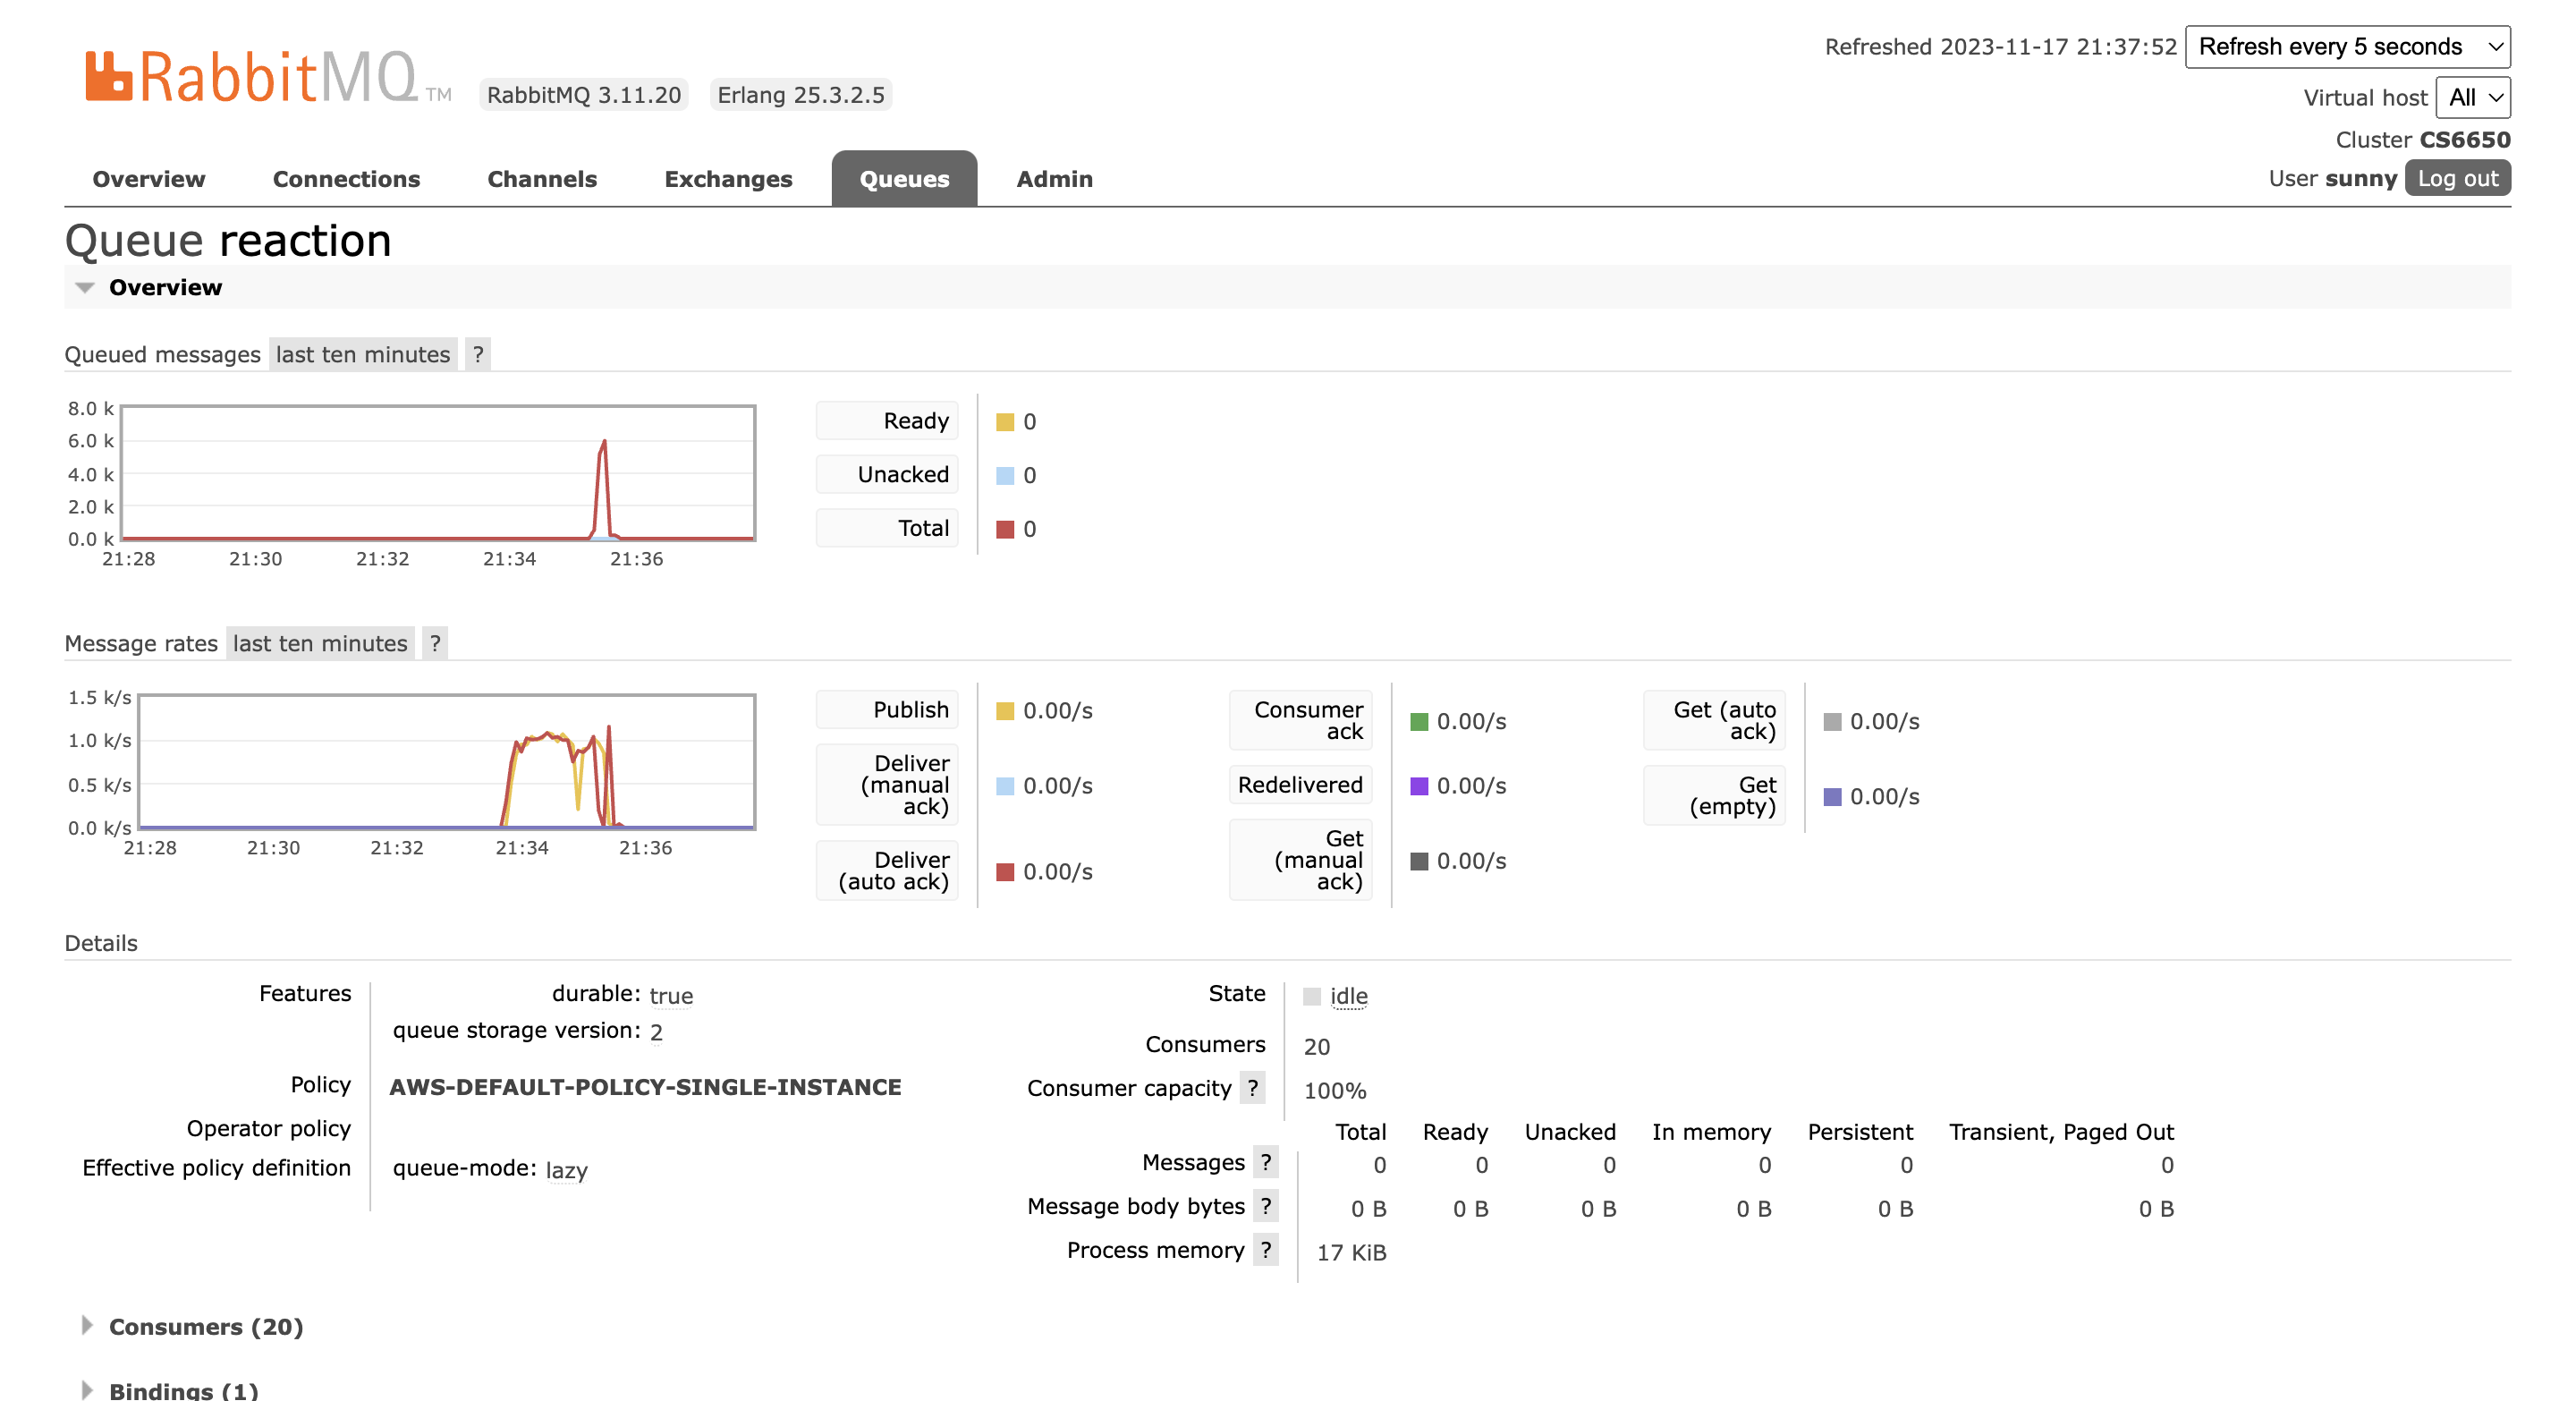
\includegraphics[width=\textwidth]{images/rabbit_mq_20consumer.png}
    \caption{MQ Console - threadGroupSize = 10, numThreadGroups = 30, delay = 2, consumers=20 (The run around 21:18)}
\end{figure}

From the console, we can spot that the consume rate is still not catching up with the producing rate, with at most 6k messages in the queue.
So I again added 10 consumers.
\begin{figure}[H]
    \centering
    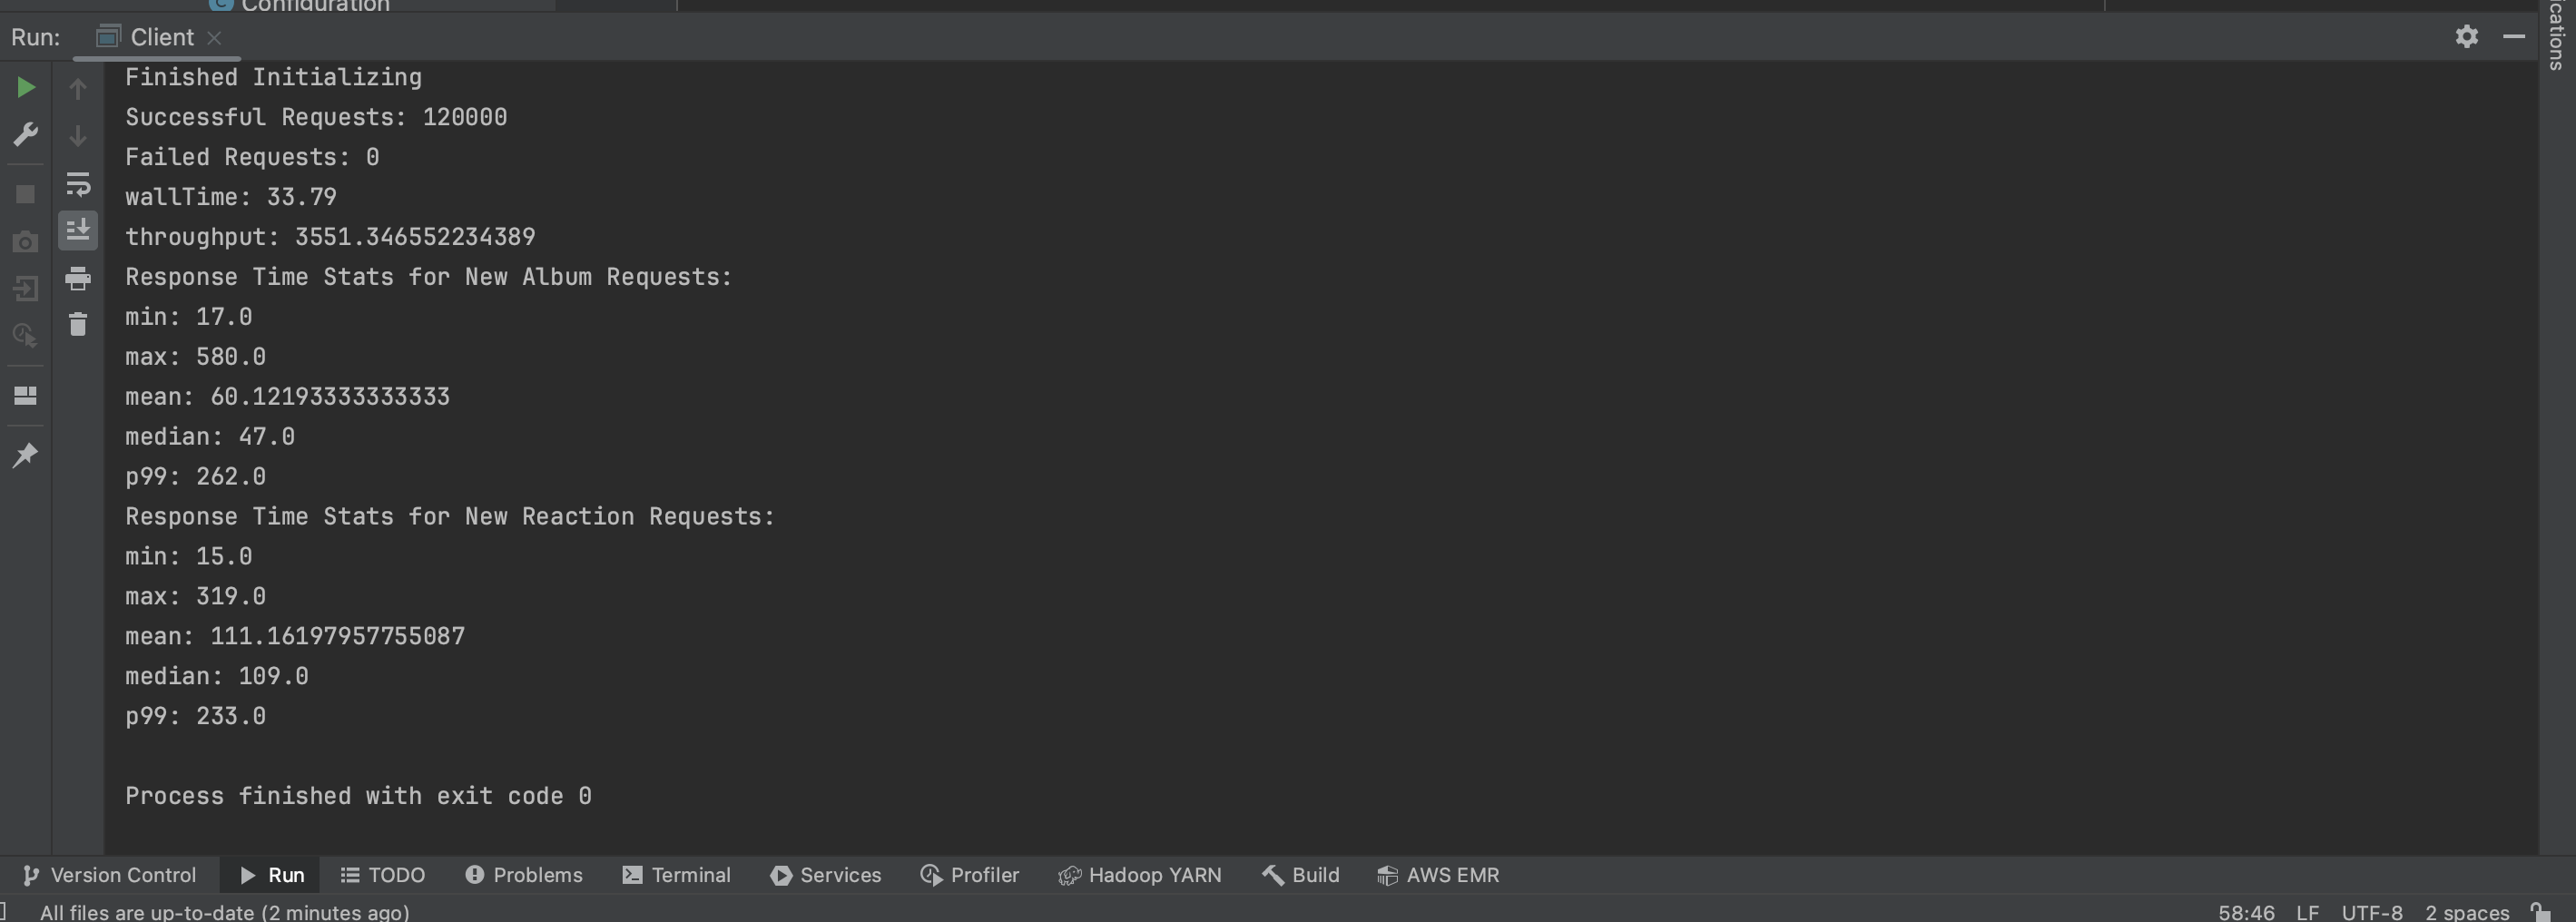
\includegraphics[width=\textwidth]{images/stats_30consumer.png}
    \caption{Single Servlet - threadGroupSize = 10, numThreadGroups = 30, delay = 2, consumers=30}
\end{figure}
\begin{figure}[H]
    \centering
    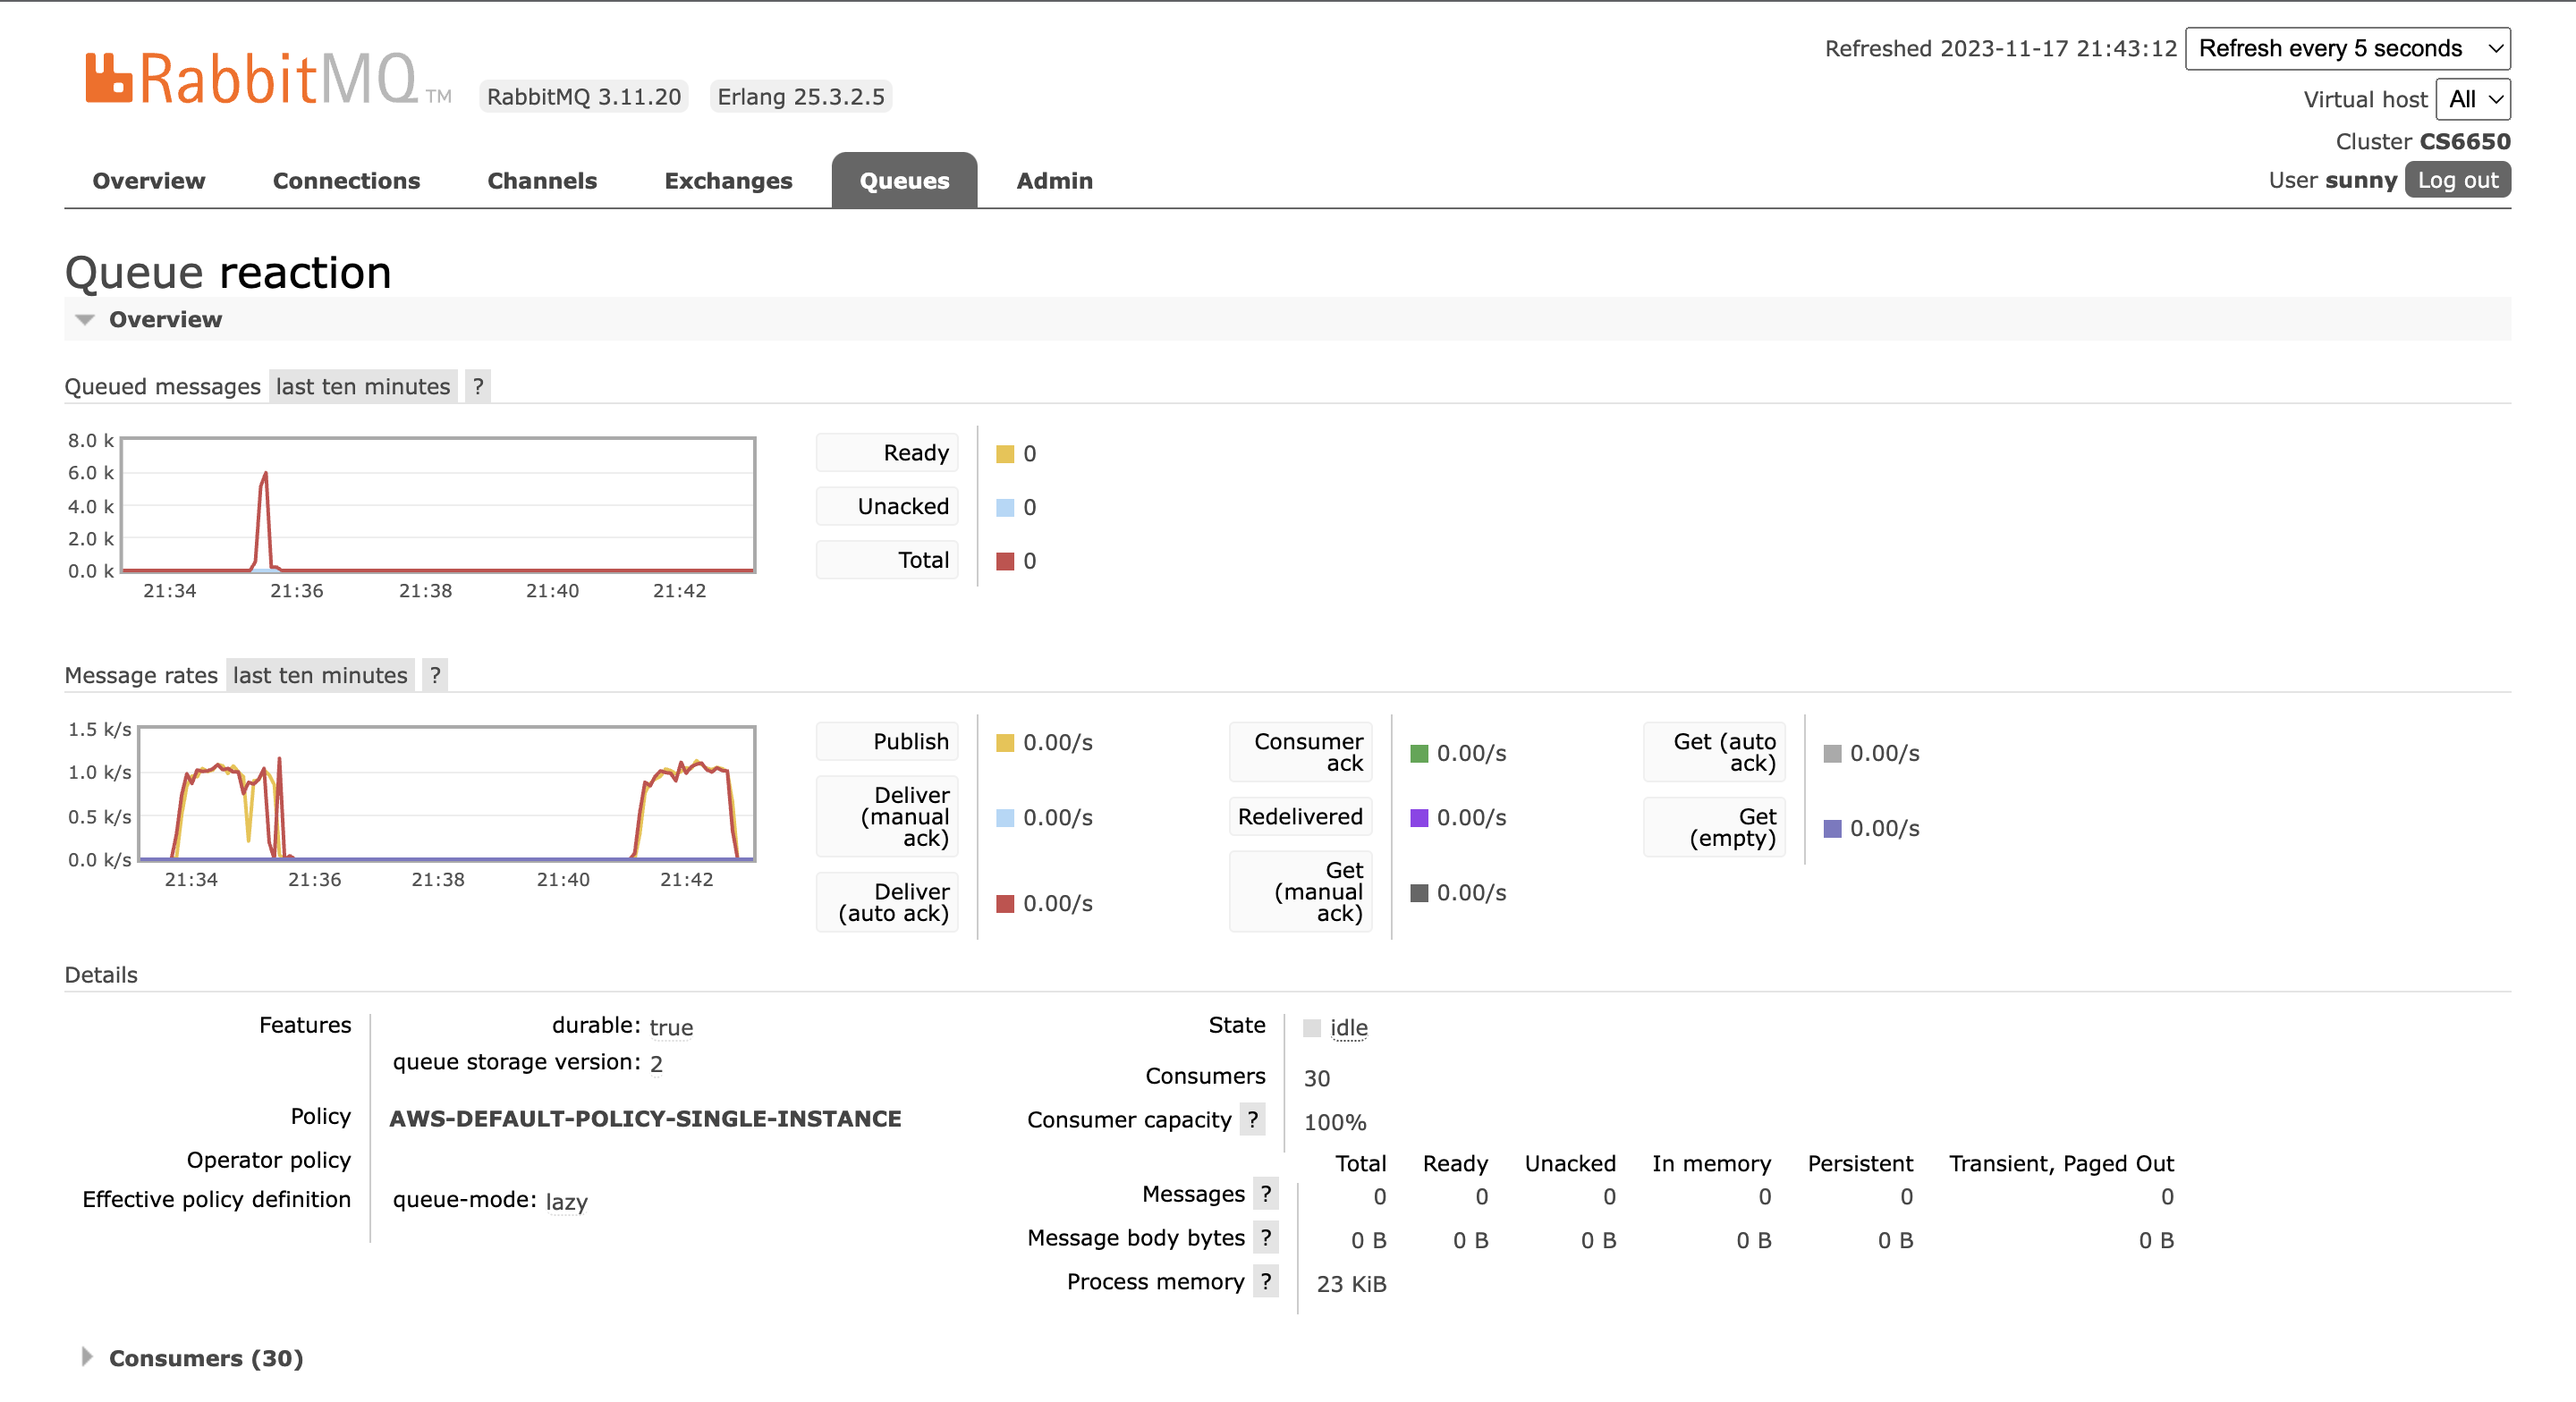
\includegraphics[width=\textwidth]{images/mq_console_30consumer.png}
    \caption{MQ Console - threadGroupSize = 10, numThreadGroups = 30, delay = 2, consumers=30}
\end{figure}

With 30 consumers, the number of messages queued in RabbitMQ is close to zero, meaning the consuming rate is greater or equal to the producing rate.
\clearpage


\end{enumerate}
\end{document}
